%Dokumentklasse
\documentclass[a4paper,12pt]{scrreprt}
\usepackage[left= 2.5cm,right = 2cm, bottom = 4 cm]{geometry}
 \usepackage[onehalfspacing]{setspace}
% ============= Packages =============

% Dokumentinformationen
\usepackage[
	pdftitle={Testautomatisierung},
	pdfsubject={},
	pdfauthor={Matthias Karl},
	pdfkeywords={}
	pdftex=true, 
	colorlinks=true,
 	breaklinks=true,
	citecolor=black,
	linkcolor=black,	
	menucolor=black,	
	urlcolor=black
]{hyperref}


% Standard Packages
\usepackage[autostyle]{csquotes}
\usepackage[utf8]{inputenc}
\usepackage[ngerman]{babel}
\usepackage[T1]{fontenc}
\usepackage{graphicx}
\graphicspath{{img/}}
\usepackage{fancyhdr}
\usepackage{lmodern}
\usepackage{color}
\usepackage{transparent}
\usepackage{caption, booktabs}
\usepackage{listings}
\usepackage{subfigure}
% \setcounter{secnumdepth}{4}
% \setcounter{tocdepth}{4} 

%code-Colour
\definecolor{javared}{rgb}{0.6,0,0} % for strings
\definecolor{javagreen}{rgb}{0.25,0.5,0.35} % comments
\definecolor{javapurple}{rgb}{0.5,0,0.35} % keywords
\definecolor{javadocblue}{rgb}{0.25,0.35,0.75} % javadoc
\definecolor{gray}{rgb}{0.5,0.5,0.5}

\lstset{frame=tb,
  language=Java,
  aboveskip=3mm,
  belowskip=3mm,
  showstringspaces=false,
  columns=flexible,
  basicstyle={\small\ttfamily},
  numbers=left,
  numberstyle=\tiny\color{gray},
  stepnumber=1,
  keywordstyle=\color{javapurple}\bfseries,
  commentstyle=\color{javagreen},
  morecomment=[s][\color{javadocblue}]{/**}{*/},
  stringstyle=\color{blue},
  breaklines=true,
  breakatwhitespace=true,
  tabsize=3
}



% zusätzliche Schriftzeichen der American Mathematical Society
\usepackage{amsfonts}
\usepackage{amsmath}

% nicht einrücken nach Absatz
\setlength{\parindent}{0pt}


% ============= Kopf- und Fußzeile =============
\pagestyle{fancy}
%
\lhead{}
\chead{}
\rhead{\slshape \leftmark}
%%
\lfoot{}
\cfoot{}
\rfoot{\thepage}
%%
\renewcommand{\headrulewidth}{0.4pt}
\renewcommand{\footrulewidth}{0pt}

% ============= Package Einstellungen & Sonstiges ============= 

%Besondere Trennungen
\hyphenation{De-zi-mal-tren-nung St-rei-fen-licht-scan-nern}
\hyphenation{Test-automatisierung}
\hyphenation{System-entwurf}

%römische Aufzählungen mit \RM{Zahl}
\newcommand{\RM}[1]{\MakeUppercase{\romannumeral #1}}


% ============= Dokumentbeginn =============

\begin{document}

\pagestyle{empty}
\begin{center}
\begin{tabular}{p{\textwidth}}


\begin{center}

\includegraphics[scale=0.17]{img/logos.jpg}
\end{center}


\\

\begin{center}
\LARGE{\textsc{
Testautomatisierung mit Selenium \\  \large{- Teilautomatisierte Generierung von Page Objects -}
}}
\end{center}

\\


\begin{center}
\large{Fakultät für Informatik und Mathematik \\
der Hochschule München \\}
\end{center}

\\

\begin{center}
\textbf{\Large{Masterarbeit}}
\end{center}



\begin{center}
vorgelegt von
\end{center}

\begin{center}
\large{\textbf{Matthias Karl}} \\
\large{Matrikel-Nr: 03280712} \\
\end{center}

\begin{center}
\large{am 29.01.2016}
\end{center}

\\

\\

\begin{center}
\begin{tabular}{lll}
\textbf{Prüfer:} & & Prof. Dr. Ullrich Hafner\\
\textbf{Zweitprüfer:} & &  Prof. Dr. Oliver Braun\\
\end{tabular}
\end{center}

\end{tabular}
\end{center}

% \part im Inhaltsverzeichnis nicht nummerieren
\makeatletter
\let\partbackup\l@part
\renewcommand*\l@part[2]{\partbackup{#1}{}}

%Seitennummerierung neu beginnen, Zahlen [arabic], röm.Zahlen [roman,Roman], Buchstaben [alph,Alph]
\pagenumbering{Roman}

\newpage
\addsec{Eidesstattliche Erklärung}
\label{erklaerung}

Hiermit versichere ich, die vorliegende Studienarbeit selbstständig und nur unter Verwendung der von mir angegebenen Quellen und Hilfsmittel verfasst zu haben. Sowohl inhaltlich als auch wörtlich entnommene Inhalte wurden als solche kenntlich gemacht. Die Arbeit hat in dieser oder vergleichbarer Form noch keinem anderem Prüfungsgremium vorgelegen. \\
\\[1.5cm]
Datum:	\hrulefill\enspace Unterschrift: \hrulefill
\\[3.5cm]
 



\addsec{Zusammenfassung / Abstract}
\label{sec:zusammenfassung}
Diese Arbeit befasst sich mit dem Themenschwerpunkt Testautomatisierung.
Zu Beginn werden zunächst die Grundlagen im Bereich der Software-Qualität und dem Testen im allgemeinen geschaffen, um dann einen Überblick über die verschiedenen Möglichkeiten der Testautomatisierung zu präsentieren.
Anhand der geschaffenen Grundlagen wird das Testautomatisierungs-Tool Selenium vorgestellt. Hierbei liegt ein besonderes Augenmerk auf dem Page Object Design Pattern. Bezüglich des Page Object Design Pattern wird eine selbst erstellte Software-Lösung vorgestellt, welche die Verwendung dieses Pattern durch eine teilautomatisierte Generierung von Page Object-Klassen vereinfachen soll.

\newpage
\pagestyle{fancy}
%Inhaltsverzeichnis
\tableofcontents

\newpage
%Seitennummerierung neu beginnen, Zahlen [arabic], röm.Zahlen [roman,Roman], Buchstaben [alph,Alph]
\pagenumbering{arabic}
% pagestyle für gesamtes Dokument aktivieren
\pagestyle{fancy}

\newpage
\chapter{Einleitung}
\label{sec:einleitung}
Software hat in der heutigen Zeit für Unternehmen und jeden einzelnen gleichermaßen an immer größer Bedeutung gewonnen.
Die Komplexität der Softwareprodukte steigt ständig weiter an. Neben der steigenden Komplexität sind auch die Anforderungen an die Qualität der Software immer weiter gewachsen.
Das hat zur Folge, dass bei der Entwicklung von Software, ein immer größeres Augenmerk auf den Bereich des Testens gelegt wird.
Um den steigenden Anforderungen an Software und Qualität bezüglich des Testens gerecht zu werden, wird häufig die Testautomatisierung als möglicher Lösungsweg vorgeschlagen.
Durch den Einsatz von Testautomatisierung verspricht man sich Vorteile beim testen von Softwarelösungen. Diese Vorteile sollen vor allem über eine Qualitäts- und Effizienzsteigerung erreicht werden.\\
Eine Vielzahl an Softwarelösungen werden heutzutage in Form von Webanwendungen umgesetzt.
Um diese automatisiert zu Testen, wird oft auf Testfälle zurückgegriffen, die automatisch Eingaben auf der Oberfläche der Anwendung tätigen, um anschließend das Verhalten der Anwendung zu überprüfen.
Ein gängiges Tool, mit welchem diese Form der Testfälle umgesetzt werden kann, ist Selenium \cite{selenium_selenium_2015}.
\\

\section{Motivation}
\label{sec:motivation}
Testautomatisierung hat oft das Problem, dass Testfälle zwar wiederholt und einfach ausgeführt werden können, der initiale Mehraufwand für die Erstellung der Testfälle aber häufig so zeitaufwändig ist, dass der erreichte Vorteil nur gering zum Tragen kommt. Ein möglicher Weg, um Verbesserungen in der Testautomatisierung zu erzielen, ist es daher, diesen Mehraufwand zu minimieren.\\
Testfälle die mit Hilfe des Selenium WebDiver entwickelt werden, leiden oftmals unter eben dieser Schwierigkeit. Die initiale Erstellung der Tests ist in der Regel sehr aufwändig.
Um die Testfälle möglichst wartbar zu halten, wird bei der Verwendung des WebDrivers ein bestimmtes Design Pattern, das Page Object Pattern, verwendet.
Bestandteil dieses Pattern ist es, eine Vielzahl von sogenannten Page Objects zu erstellen, welche die einzelnen Seiten einer Webanwendung repräsentieren.\\
In Hinblick auf den initialen Mehraufwand weist die Erstellung dieser Page Object-Klassen ein großes Einsparungspotential auf. Aufgrund ihrer generischen Struktur bieten die Page Objects nämlich das Potential automatisch erzeugt zu werden.
In Zusammenarbeit mit dem IT-Dienstleister der Landeshauptstadt München (it@M) soll daher eine Software entwickelt werden, mit deren Hilfe die Erstellung der Page Object-Klassen vereinfacht werden kann.

\section{Roadmap}
\label{roadmap}
Der Hauptteil dieser Arbeit gliedert sich in vier Kapitel. In Kapitel \ref{sec:grundlagen} werden zunächst die Grundlagen in den Bereichen der Software-Qualität, dem Testen im allgemeinen und der Testautomatisierung im speziellen gelegt.
Kapitel \ref{sec:testautomatisierung} geht näher auf die Testautomatisierung ein und soll einen Überblick über die verschiedenen Bereiche und Möglichkeiten geben, welche die Testautomatisierung bietet.
In Kapitel \ref{sec:selenium} wird das Testautomatisierungstool Selenium vorgestellt und in diesem Zusammenhang das Page Object Pattern erläutert.
In Kapitel \ref{sec:teilautomatisierte_generierung_von_pageObjects} wird eine Softwarelösung vorgestellt mit deren Hilfe die Verwendung des Page Object Pattern unterstützt wird.

  





\newpage
\chapter{Grundlagen}
\label{sec:grundlagen}


\section{Software-Qualität}
\label{sec:softwarequalität}

Nahezu jeder Programmierer ist schon einmal mit dem Begriff der Software-Qualität in Berührung gekommen. Diesen Qualitätsbegriff jedoch genau zu erfassen, erweist sich als schwierig.
Die DIN-ISO-Norm 9126 definiert Software-Qualität wie folgt:
\\
\glqq Software-Qualität ist die Gesamtheit der Merkmale und Merkmalswerte eines Software-Produkts, die sich auf dessen Eignung beziehen, festgelegte Erfordernisse zu erfüllen.\grqq \cite{iso/iec_iso/iec_2001}
\\
Im Jahr 2005 ist die DIN-ISO-Norm 9126 von der DIN-ISO-Norm 25010 \cite{iso/iec_iso/iec_2011} abgelöst worden. Die Definition der neuen Norm unterscheidet sich von der alten Definition vor allem darin, dass nun die Erfüllung von Benutzerbedürfnissen und nicht mehr die Erfüllung von Erfordernissen im Vordergrund steht.\\
Folgt man der Analyse von Hoffmann \cite[vgl. S.6 ff.]{hoffmann_software-qualitat_2013} wird deutlich, dass es sich bei dem Begriff der Software-Qualität um eine multikausale Größe handelt. Das bedeutet, dass zur Bestimmung der Qualität einer Software nicht nur ein einzelnes Kriterium existiert. Vielmehr verbergen sich hinter dem Begriff eine ganze Reihe verschiedener Kriterien, die je nach den gestellten Anforderungen in ihrer Relevanz variieren.
Sammlungen solcher Kriterien werden in sogenannten Qualitätsmodellen zusammengefasst. Die DIN-ISO-Norm 25010 \cite{iso/iec_iso/iec_2011} bietet ein solches Qualitätsmodell und definiert damit eine Reihe von wesentlichen Merkmalen, die für die Beurteilung der Software-Qualität eine Rolle spielen. Die Merkmale der DIN-ISO-Norm 25010 \cite{iso/iec_iso/iec_2011} sind in Abbildung \ref{fig:qualitaetsmerkmaleVonSoftwaresystemen} zusammengefasst.
\begin{figure}[htb]
  \centering  
  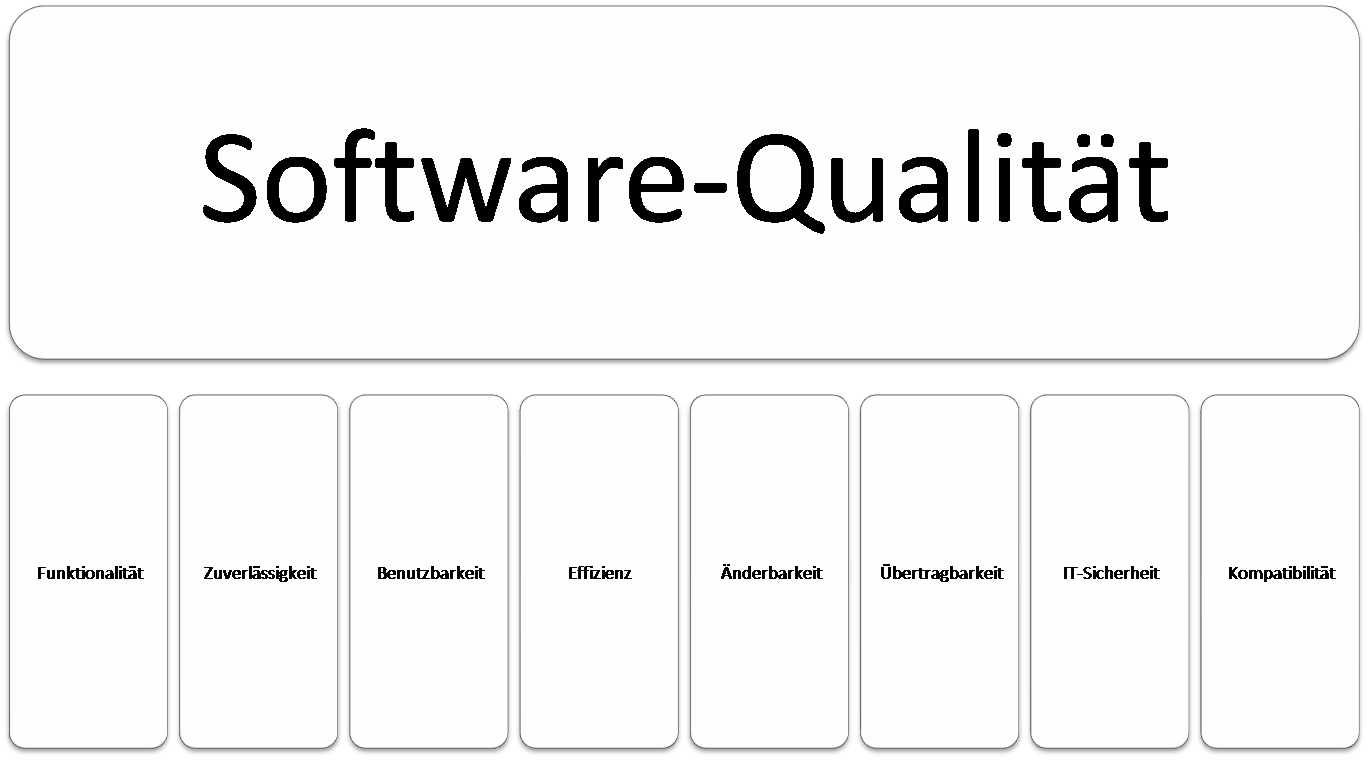
\includegraphics[scale=0.7]{img/softwarequalitaet25010.png}\\
  \footnotesize\sffamily\textbf{Quelle:} \cite{iso/iec_iso/iec_2011}
  \caption{Qualitätsmerkmale von Softwaresystemen (ISO 25010)}
  \label{fig:qualitaetsmerkmaleVonSoftwaresystemen}
\end{figure}
Eine nähere Definition der einzelnen Begriffe des Qualitätsmodells kann beispielsweise dem Buch \grq Software-Qualität\grq\ von Dirk W. Hoffmann \cite[S.7 ff.]{hoffmann_software-qualitat_2013} entnommen werden.\\
Um die Qualität einer Software zu steigern, bietet die moderne Software-Qualitätssicherung laut Hofmann \cite[vgl. S.19 ff.]{hoffmann_software-qualitat_2013} eine Vielzahl von Methoden und Techniken:
Ein Teil der Methoden versucht durch eine Verbesserung des Prozesses der Produkterstellung die Entstehung von qualitativ hochwertigen Produkten zu begünstigen. Diese Methoden fallen in den Bereich der Prozessqualität.
Einen weiteren Bereich bilden die Methoden, die zur Verbesserung der Produktqualität dienen. Bei diesen Methoden wird das Softwareprodukt direkt bezüglich der Qualitätsmerkmale überprüft. Dieser Bereich unterteilt sich in die konstruktive und analytische Qualitätssicherung. Unter konstruktiver Qualitätssicherung versteht man z.B. den Einsatz von Methoden, Werkzeugen oder Standards, die
dafür sorgen, dass ein Produkt bestimmte Forderungen erfüllt. 
Unter analytischer Qualitätssicherung versteht man den Einsatz von analysierenden bzw. prüfenden Verfahren, die Aussagen
über die Qualität eines Produkts machen.
In diesem Bereich der Qualitätssicherung befindet sich unter anderem der klassische Software-Test. Eine Übersicht über das gesamte Gebiet der Software-Qualitätssicherung, wie es sich uns gegenwärtig darstellt, ist in Abbildung \ref{fig:softwareQualitätssicherung} dargestellt. 
\begin{figure}[htb]
  \centering  
  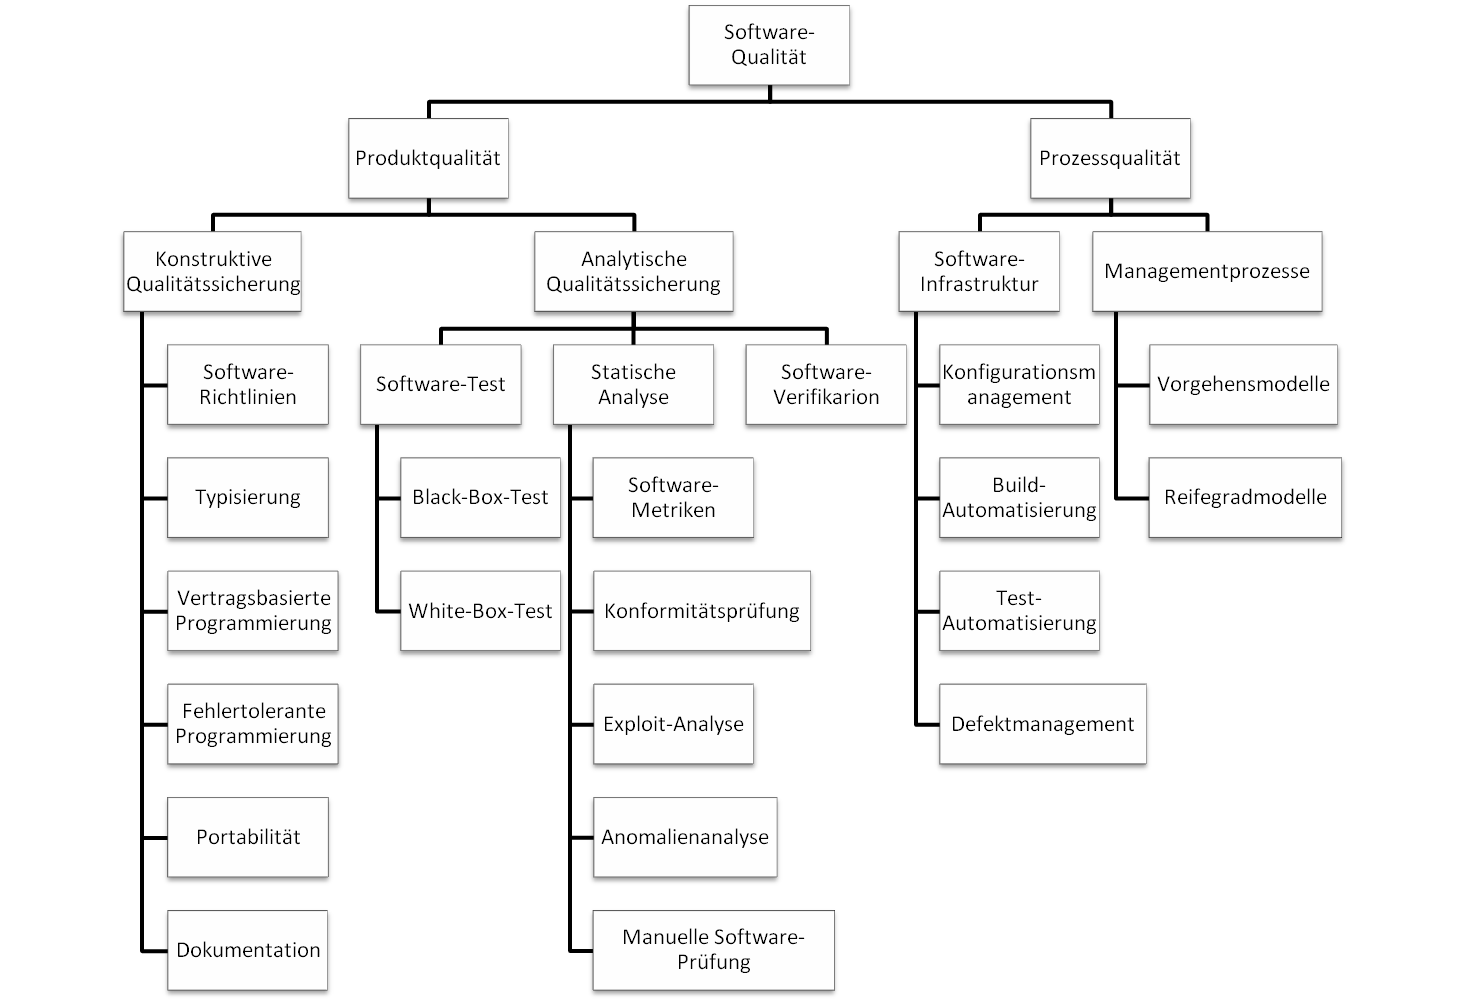
\includegraphics[scale=0.7]{img/softwarequalitaet.png}\\
  \footnotesize\sffamily\textbf{Quelle:} \cite[vgl. S.20]{hoffmann_software-qualitat_2013}
  \caption{Übersicht über das Gebiet der Software-Qualitätssicherung}
  \label{fig:softwareQualitätssicherung}
\end{figure}



\section{Softwaretest}
\label{sec:softwaretest}
Im Laufe der Zeit wurden viele Versuche unternommen, um die Qualität von Software zu steigern. Besondere Bedeutung hat hierbei der Software-Test erlangt.
Der IEEE Standard 610.12 definiert den Begriff Test als das Ausführen einer Software unter bestimmten Bedingungen mit dem Ziel, die erhaltenen Ergebnisse auszuwerten, also gegen erwartete Werte zu vergleichen.
(Im Original: \glqq An activity in which a system or component is executed under specific conditions, the results are observed or recorded, and an evaluation is made of some aspect of the system or component.\grqq\ \cite{ieee_ieee_1991})\\
Bereits zu Beginn der Softwareentwicklung wurde versucht, Programme vor ihrer Auslieferung zu testen. Der dabei erzielte Erfolg entsprach nicht immer den Erwartungen. Im Laufe der Jahre wurde das Testen daher auf eine immer breitere Grundlage gestellt. Es entwickelten sich Unterteilungen des Software-Tests, die bis heute Bestand haben. Thaller \cite[vgl. S.18]{thaller_software-test_2002} nennt hier beispielsweise:
\begin{itemize}
\item White-Box-Test
\item Black-Box-Test und externe Testgruppe
\item Volume Test, Stress Test und Test auf Systemebene
\end{itemize}
Jeder dieser Begriffe beschreibt bestimmte Techniken, die bei konsequenter Anwendung dazu führen können, Fehler in Softwareprodukten zu identifizieren. 

Nach Hoffmann \cite[vgl. S.22]{hoffmann_software-qualitat_2013} spielt neben der Auswahl der richtigen Techniken für ein bestimmtes Problem in der Praxis die Testkonstruktion eine zentrale Rolle. Bereits für kleine Programme ist es faktisch nicht mehr möglich das Verhalten der Software für alle möglichen Eingaben zu überprüfen. Es muss sich daher immer auf eine vergleichsweise geringe Auswahl an Testfällen beschränkt werden. Testfälle unterscheiden sich jedoch stark in ihrer Relevanz. Die Auswahl der Testfälle hat daher einen großen Einfluss auf die Anzahl der gefundenen Fehler und damit auch auf die Qualität des Endprodukts. 

Laut Hofmann \cite[vgl. S.22]{hoffmann_software-qualitat_2013} ist der Software-Test eine der verbreitetsten Techniken zur Verbesserung der Software-Qualität. Um über lange Sicht gute Software produzieren zu können, reicht es jedoch nicht aus, sich nur auf eine Technik der Software-Qualitätssicherung zu stützen. Ein großer Nachteil des Software-Tests ist laut Thaller \cite[vgl. S.18]{thaller_software-test_2002}, dass Fehler erst in einer relativ späten Phase der Entwicklung identifiziert werden. Je später ein Fehler jedoch erkannt wird, desto teurer wird auch seine Beseitigung. Abbildung \ref{fig:softwareQualitätssicherung} zeigt, dass der Software-Test nur eine von vielen Techniken des Qualitätsmanagement darstellt. Um eine möglichst qualitativ hochwertige Software zu erhalten, ist es daher ratsam, sich bei der Qualitätssicherung möglichst breit aufzustellen und sich nicht nur auf die analytische Qualitätssicherung in Form des Software-Tests zu verlassen. 


\section{Testautomatisierung}
\label{sec:testautoGrundlagen}
Das Testen von Software macht in heutigen Projekten einen großen Teil der Projektkosten aus. So sprechen beispielsweise Harrold \cite{harrold_testing:_2000} und auch Ramler \cite{ramler_economic_2006} davon, dass das Testen für 50\% 
und mehr der gesamten Projektkosten verantwortlich sein kann. 
Mit steigender Komplexität der Software müssen, um eine konstante Qualität der Software zu gewährleisten, immer höhere Ausgaben für das Testen getätigt werden.  
Um diese Kosten zu reduzieren, haben sich im Laufe der Zeit die bestehenden Testmethoden immer weiter entwickelt und auch neue Ansätze herausgebildet. Harrold \cite{harrold_testing:_2000} beschreibt als einen Ansatz, Software-Tests möglichst automatisiert durchzuführen. Diesen Ansatz fast man mit dem Begriff Testautomatisierung zusammen.
Seidl et al. \cite[S.7]{seidl_basiswissen_2012} definieren Testautomatisierung als \glqq die Durchführung von ansonsten manuellen Testtätigkeiten durch Automaten.\grqq\
Diese Definition zeigt, dass das Spektrum der Testautomatisierung breit gefächert ist. Testautomatisierung beschränkt sich nicht nur auf das automatisierte Durchführen von Testfällen, sondern erstreckt sich über alle Bereiche des Software-Tests. Die verschiedenen Möglichkeiten der Testautomatisierung werden in Kapitel \ref{sec:bereiche_der_testautomatisierung} dargestellt.
Aus Sicht des Qualitätsmanagement ist die Testautomatisierung sowohl den Methoden zur Steigerung der Produktqualität als auch der Prozessqualität zugeordnet. Ein automatisierter Software-Test hat immer noch den selben Charakter wie ein manueller Software-Test und ist daher ein Teil der analytischen Qualitätssicherung. Allerdings erfordert Testautomatisierung laut Hoffmann \cite[vgl. Seite 25]{hoffmann_software-qualitat_2013} auch immer infrastrukturelle Anpassungen. Automatisierte Testfälle benötigen in der Regel eine besondere Software-Infrastruktur, wie etwa ein Automatisierungsframework. Solche Maßnahmen, die den Programmentwickler aus technischer Sicht in die Lage versetzen, seiner täglichen Arbeit in geregelter und vor allem produktiver Weise nachzugehen, werden den Methoden zur Verbesserung der Prozessqualität zugeordnet (siehe Abbildung \ref{fig:softwareQualitätssicherung}).



\section{Testprozess}
\label{sec:testprozess}

Um Software-Tests effektiv und strukturiert durchzuführen, wird ein feiner Ablaufplan für die einzelnen Testaufgaben benötigt. Diesen Ablaufplan fassen Splinner und Linz \cite{spillner_basiswissen_2007} im fundamentalen Testprozess zusammen. Die einzelnen Arbeitsschritte, die im Lebenszyklus eines Software-Tests anfallen, werden dabei verschiedenen Phasen zugeordnet.
Durch den Testprozess wird die Aufgabe des Testens in kleinere Testaufgaben untergliedert.

Testaufgaben, die Splinner und Linz \cite{spillner_basiswissen_2007} dabei unterscheiden sind:

\begin{itemize}
	  \itemsep0pt
      \item Testplanung und Steuerung
      \item Testanalyse und Testdesign
      \item Testrealisierung und Testdurchführung
      \item Testauswertung und Bericht
      \item Abschluss der Testaktivitäten       
\end{itemize}

Laut Seidl et al. \cite[S. 9]{seidl_basiswissen_2012} wird jeder, der strukturiert testet, diese Aktivitäten auf die eine oder andere Weise abbilden.\\
Splinner und Linz \cite[S.19]{spillner_basiswissen_2007} geben zu bedenken, dass obgleich die Aufgaben in sequenzieller Reihenfolge im Testprozess angegeben sind, sie sich trotzdem überschneiden können und teilweise auch gleichzeitig durchgeführt werden. \\ Auf Grundlage des fundamentalen Testprozesses nach Splinner und Linz \cite[S.20ff]{spillner_basiswissen_2007} werden im Folgenden die Teilaufgaben näher beschrieben. 
Diese Beschreibung wird durch Ausführungen von Seidl et al. \cite[S. 9 ff.]{seidl_basiswissen_2012}, vor allem bezüglich der Testautomatisierung, erweitert. 

\subsection{Testplanung und Steuerung}
\label{subsec:testplanung_und_steuerung}
Um dem Umfang und der Komplexität heutiger Software-Tests gerecht zu werden, benötigt man zu Beginn des Testprozesses eine genaue Planung.
Ziel dieser Planung ist es, den Rahmen für die weiteren Testaktivitäten festzulegen. Die Aufgaben und die Zielsetzungen der Tests müssen ermittelt wurden. Eine Ressourcenplanung wird benötigt und eine geeignete Teststrategie muss ermittelt werden. In Kapitel \ref{sec:softwaretest} wurde bereits erwähnt, dass das vollständige Testen einer Anwendung in der Regel nicht möglich ist. Die einzelnen Systemteile müssen daher nach Schwere der zu erwartenden Fehlerwirkung priorisiert werden. Um so schwerwiegender die zu erwartende Fehlerwirkung ist, um so intensiver muss der betrachtete Systemteil auch getestet werden. Ziel der Teststrategie ist also \glqq die optimale Verteilung der Tests auf die \frqq richtigen\flqq\ Stellen des Softwaresystems.\grqq\ \cite[S.21]{spillner_basiswissen_2007} \\ Steht das Softwareprojekt unter einem hohen Zeitdruck, müssen Testfälle zusätzlich priorisiert werden.
Um zu verhindern, dass das Testen zu einem endlosen Prozess wird, werden geeignete Testendekriterien festgelegt. Anhand dieser Kriterien kann später entschieden werden, ob der Testprozess abgeschlossen werden kann.

Bereits zu Beginn des Testprozesses werden auch wichtige Grundsteine für eine spätere Testautomatisierung gelegt. Es muss entschieden werden, in welchen Teststufen und Testbereichen eine Automatisierung eingesetzt werden soll. Vor allem ist die Frage zu klären, ob und in welchem Ausmaß eine Automatisierung überhaupt sinnvoll ist. Es kann durchaus vorkommen, dass eine Analyse ergibt, dass eine Testautomatisierung für ein Projekt unwirtschaftlich ist.
Entscheidet man sich für eine Testautomatisierung, hat das in der Regel große Auswirkungen auf die einzusetzenden Ressourcen und die zeitliche Planung und Aufwandsschätzung.
Oftmals wird im Rahmen der Tests eine besondere Werkzeugunterstützung oder Infrastruktur benötigt. Derartige Punkte müssen auch bereits in der frühen Planungsphase berücksichtigt werden.

Die gesamten erarbeiteten Rahmenbedingungen werden in einem Testkonzept dokumentiert.
Eine mögliche Vorlage für dieses Dokument bietet die internationale Norm IEEE 829-2008 \cite{ieee_ieee_2008}.
Neben der frühzeitigen Planung der Tests muss während des gesamten Testprozesses eine Steuerung erfolgen.
Hierfür werden die Ergebnisse und Fortschritte der Tests und des Projekts laufend erhoben, geprüft und bewertet. Werden Probleme erkannt, kann so rechtzeitig gegengesteuert werden. 

\subsection{Testanalyse und Testdesign}
\label{subsec:testanalyse_und_design}
In dieser Phase wird zunächst die Qualität der Testbasis überprüft. Alle Dokumente, die für die Erstellung der Testfälle benötigt werden, müssen in ausreichendem Detailgrad vorhanden sein. Mit Hilfe der qualitätsgesicherten Dokumente kann die eigentliche Testfallerstellung beginnen.
Anhand der Informationen aus dem Testkonzept und den Spezifikationen, werden mittels strukturierter Testfallerstellungsmethoden logische Testfälle erstellt. Diese logischen Testfälle können dann in einer späteren Phase konkretisiert werden, indem ihnen z.B. tatsächliche Eingabewerte zugeordnet werden. Für jeden Testfall müssen die möglichen Rand- und Vorbedingungen sowie ein erwartetes Ergebnis bestimmt werden.\\
In dieser Phase beginnen auch erste Aufgaben, die mit der Testautomatisierung in Zusammenhang stehen.
Abgestimmt auf die ausgewählten Automatisierungswerkzeuge und die zu testende Software, muss die Umgebung für die Testautomatisierung vorbereitet werden. Anhand der Vorgaben des Testkonzeptes können dann jene Testfälle und Testabläufe ausgewählt werden, die im Zuge der Testautomatisierung implementiert werden sollen. Hierbei wird noch einmal die technische Umsetzbarkeit geprüft. Bei der Auswahl der Testfälle sollte zu Beginn eine möglichst breite Testabdeckung angestrebt werden.
Problemfelder können dann später durch weitere Testfälle in der Tiefe getestet werden.

\subsection{Testrealisierung und Testdurchführung}
\label{subsec:testrealisierung_und_durchführung}
In diesem Schritt des Testprozesses werden aus den logischen Testfällen der vorangegangenen Phase konkrete Testfälle gebildet.
Diese werden anhand ihrer fachlichen und technischen Zusammengehörigkeit zu Testszenarien gruppiert und anhand der Vorgaben aus dem Testkonzept priorisiert.
Sobald die zu testende Software zur Verfügung steht, kann mit der Abarbeitung begonnen werden. Die dabei erhaltenen Ergebnisse werden vollständig protokolliert. Werden im Zuge der Durchführung Fehler aufgedeckt, muss darauf in geeigneter Weise reagiert werden. Es kann beispielsweise ein zuvor definierter Fehlerprozess gestartet werden.
Korrekturen und nachgehende Veränderungen am Testobjekt werden durch eine Wiederholung der Testläufe abgedeckt.\\
Aus Sicht der Testautomatisierung beginnt in dieser Phase die technische Umsetzung.
In vielen Fällen bedeutet das Programmiertätigkeit. Diese Programmiertätigkeiten sind wiederum anfällig für eigene Fehler und müssen daher in angemessener Weise selbst qualitätsgesichert werden. Auch bei der Testautomatisierung ist eine Zusammenfassung von Testfällen sinnvoll. Auf diese Weise kann man funktionalen und logischen Abhängigkeiten zwischen den Testfällen gerecht werden.
Nach der Implementierung können die geplanten Testfälle durchgeführt werden.
Gerade bei der Automatisierung ist eine genaue Protokollierung der Ergebnisse besonders wichtig.
Nur dadurch ist es später möglich, aufgetretene Fehler überhaupt zu lokalisieren.


\subsection{Testauswertung und Bericht}
\label{subsec:testauswertung_und_bericht}
In dieser Phase des Prozesses wird geprüft, ob die im Testkonzept definierten Testendekriterien erreicht wurden. Sind alle Forderungen erfüllt, kann es zu einem Abschluss der Testaktivitäten kommen. Kommt es zu Abweichungen im Bezug auf diese Kriterien, muss darauf entsprechend reagiert werden. Es können Fehlerkorrekturen durchgeführt werden oder neue Testfälle erstellt werden. Aber auch der umgekehrte Fall ist möglich. Es kann dazu kommen, dass Endekriterien nur mit unverhältnismäßig hohem Aufwand erreicht werden 
und daher bestimmte Testfälle entfallen oder Kriterien überdacht werden müssen.

Für die Testautomatisierung ist die wesentliche Aufgabe dieser Phase die Auswertung und Aufarbeitung der erhaltenen Ergebnisse. Automatisierte Tests generieren oftmals eine Fülle an Log-Dateien und Protokollen. Um aus diesen Ergebnissen die richtigen Schlüsse zu ziehen und sie für Dritte zugänglich zu machen, müssen sie in eine lesbare Form gebracht werden.

In jedem Fall muss über die erhaltenen Ergebnisse und das daraus resultierende Vorgehen ein Testbericht erstellt werden. Je nach Umfang und Phase der Tests kann dieser mehr oder weniger formal ausfallen. Für einen Komponententest reicht beispielsweise eine formlose Mitteilung. Höhere Teststufen erfordern einen formaleren Bericht.



\subsection{Abschluss der Testaktivitäten}
\label{subsec:abschluss_der_testaktivitäten}
Sind die Testaktivitäten beendet, sollten zum Schluss alle im Laufe des Testprozesses gemachten Erfahrungen analysiert werden. So können die gewonnenen Erkenntnisse für spätere Projekte genutzt werden. Dadurch kann eine stetige Verbesserung des Testprozesses erreicht werden.
Die während des Prozesses erstellten Testfälle, sowie alle sonstigen Ergebnisse, sollten archiviert werden. Auf diese Weise stehen sie für folgende Regressionstests zur Verfügung. Die Kosten für Wartung und Pflege der Software können damit gesenkt werden.
Bei der Testautomatisierung bedeutet das, die Wiederherstellbarkeit der Testumgebung und des Sourcecodes sicherzustellen.
\newline\\
Abschließend ist zu sagen, dass sich die Testautomatisierung in der Regel gut in einen bereits bestehenden Testprozess integrieren lässt. Sie wird allerdings \glqq den Prozess nicht verbessern oder gerade richten, sondern nur unterstützen.\grqq\ \cite[S.21]{seidl_basiswissen_2012} \\ Ist der Testprozess schon vor Einführung einer Automatisierung schlecht organisiert gewesen, wird er sich nach der Einführung nicht verbessern.
Die Testautomatisierung ist also nicht als Heilmittel für schlecht laufende Prozesse gedacht, sondern als Möglichkeit einen bereits gut etablierten Prozess effizienter und effektiver zu gestalten.

\section{Vorgehensmodelle}
\label{sec:vorgehensmodelle}
Der in Kapitel \ref{sec:testprozess} beschriebene Testprozess ist nicht als losgelöster, eigenständiger Prozess zu betrachten. Vielmehr ist der Testprozess immer ein Teil eines größeren Entwicklungsablaufes bei der Erstellung eines Softwareproduktes. Einen solchen Entwicklungsablauf versucht man mit Hilfe von sogenannten Softwareentwicklungsmodellen, auch Vorgehensmodelle genannt, abzubilden.
Ein Projekt wird dazu in einzelne Phasen untergliedert, an deren Ende ein gewisses Ziel bzw. Ergebnis steht.
Auf gröbster Ebene lassen sich die Abläufe auf vier Hauptphasen reduzieren. Diese Phasen finden sich mehr oder weniger ausgeprägt in den meisten der gängigen Vorgehensmodelle wieder und werden auch so von Seidl et al. \cite[S.21 ff.]{seidl_basiswissen_2012} verwendet:

\begin{itemize}
\item Spezifikation
\item Design
\item Entwicklung
\item Test
\end{itemize}

Das Testen, bzw. der Testprozess ist eine von mehreren Phasen in einem solchen Entwicklungsmodell.
Es gibt eine Vielzahl von unterschiedlichen Softwareentwicklungsmodellen. Der Hauptunterschied liegt meist in der zeitlichen Koppelung und der inhaltlichen Ausprägung der einzelnen Phasen. Die einzelnen Phasen können sich innerhalb eines Vorgehensmodells überschneiden und wiederholen und müssen auch nicht immer, wie in der Auflistung angegeben, sequenziell abgearbeitet werden.
Aus der Sicht der Testautomatisierung ist nach Seidl et al. \cite[vgl. S.21 ff.]{seidl_basiswissen_2012} eine Einteilung der verschiedenen Vorgehensmodelle in zwei Gruppen sinnvoll: 

\begin{itemize}
\item Klassische Entwicklungsmodelle, die eher sequentiell ausgerichtet sind
\item Iterative und agile Entwicklungsmodelle, die sich durch Parallelisierung und kurze Iterationen auszeichnen.
\end{itemize}

\subsection{Klassische Entwicklungsmodelle}
\label{subsec:klassische_entwicklungsmodelle}

Die hier als klassische Entwicklungsmodelle betitelten Vorgehensmodelle zeichnen sich vor allem dadurch aus, dass die einzelnen Phasen sequenziell ausgeführt werden. Der bekannteste Vertreter dieser Vorgehensmodelle ist das Wasserfallmodell \cite{royce_managing_1987}. In diesem Modell sind alle Phasen strikt voneinander getrennt. Eine neue Phase kann erst begonnen werden, wenn eine vorangegangene Phase abgeschlossen wurde. Rücksprünge in vorangegangenen Phasen sind unerwünscht. In der Praxis wird dieses Vorgehen, laut Seidl et al. \cite[vgl. S.22]{seidl_basiswissen_2012}, jedoch oft nicht ganz so strikt umgesetzt. Es kommt zu Mischformen, bei denen die einzelnen Phasen nicht mehr voll sequenziell abgearbeitet werden, sondern sich teilweise überlagern. Vor allem im Bereich des Testens geht man oft zu einer solchen Mischform über. Das Testen ist meist keine getrennte Phase am Ende des Entwicklungsprozesses, sondern erstreckt sich über den gesamten Prozess ausgehend von der frühen Spezifikationsphase. Mögliche Ausprägungen klassischer Entwicklungsmodelle sind in Abbildung \ref{fig:verschiedene_auspraegungen_klassischer_entwicklungsmodelle} dargestellt.

\begin{figure}[htb]
  \centering  
  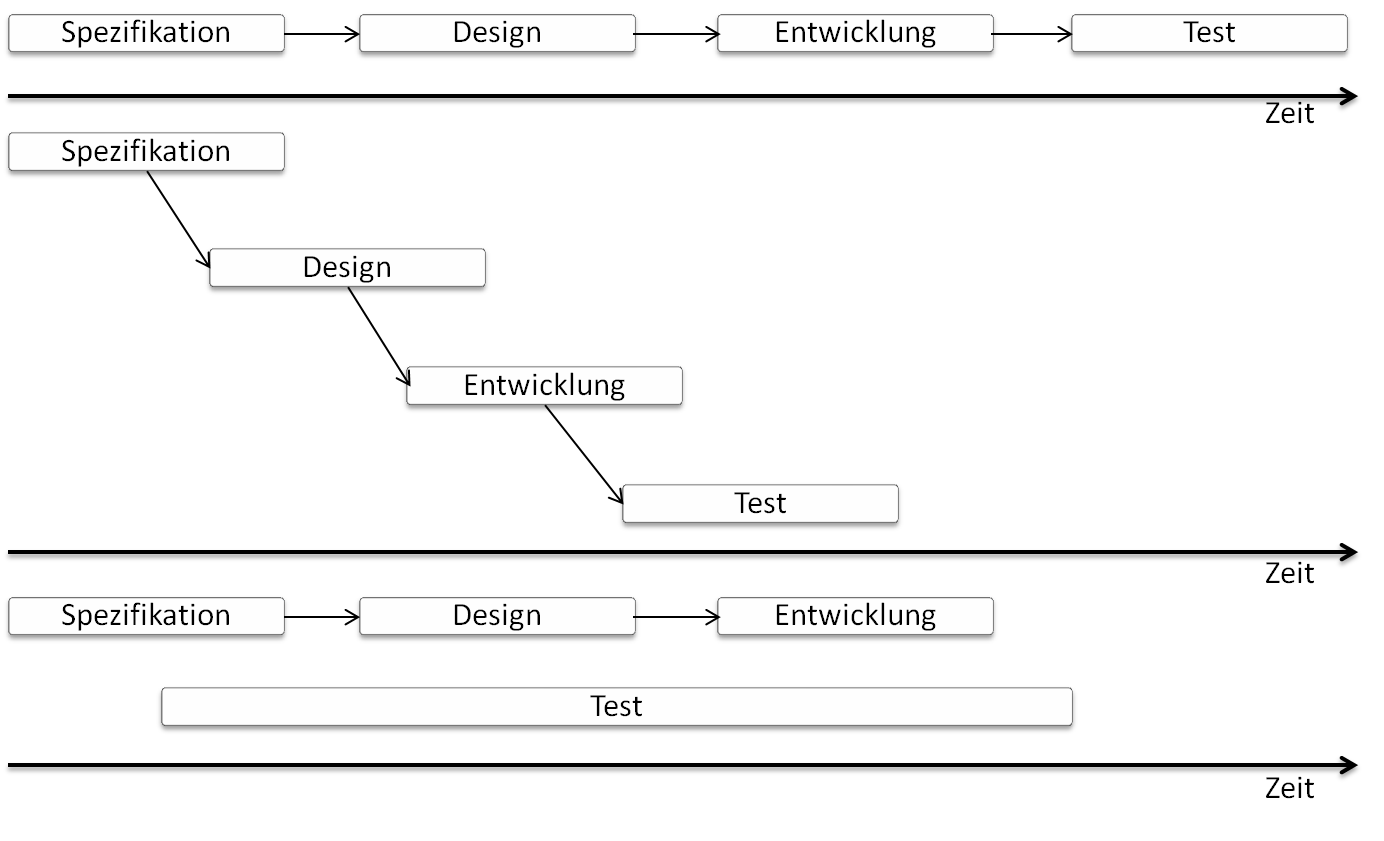
\includegraphics[scale=0.7]{img/sequentielleentwicklungsmodelle.png}\\
  \footnotesize\sffamily\textbf{Quelle:} \cite[vgl. S.22]{seidl_basiswissen_2012}
  \caption{Verschiedene Ausprägungen klassischer Entwicklungsmodelle}
  \label{fig:verschiedene_auspraegungen_klassischer_entwicklungsmodelle}
\end{figure}

Seidl et al. \cite[vgl. S.22]{seidl_basiswissen_2012} stellen fest, dass in Projekten, in denen ein sequenzielles Vorgehen gewählt wird, bereits in der frühen Planungsphase des Testprozesses genau abzuwägen ist, ob eine Automatisierung der Testfälle überhaupt sinnvoll ist.
Wenn zu Beginn des Projektes schon klar ist, dass die Testfälle nur ein einziges Mal, am Ende des Entwicklungsprozesses, ausgeführt werden, steht eine Automatisierung oft nicht in Relation zu den erhöhten Kosten, die bei der Erstellung der Tests anfallen würden.
Es ist allerdings zu beachten, dass Software meist mit dem Ende eines Projektes nicht seinen finalen Stand erreicht hat. Fehler sowie geänderte Anforderungen führen meist dazu, dass sich Softwareprodukte ständig weiterentwickeln.
Diese Weiterentwicklung ist zwangsläufig mit Codeänderungen verbunden, die wiederum zu Fehlern in bereits bestehendem Code führen können.
Um solche Fehler zu entdecken müssen im Rahmen von Regressionstests auch Testfälle wiederholt werden, die bereits erfolgreich abgeschlossen wurden.
Solche Regressionstests lassen sich bei einer vorhandenen Testautomatisierung besonders leicht durchführen. Sind also in der Software nach Projektabschluss größere Änderungen zu erwarten, kann sich eine Automatisierung über längere Sicht durchaus lohnen.
Neben Regressionstests kann nach Seidl et al. \cite[vgl. S.23]{seidl_basiswissen_2012} auch die Notwendigkeit einer höheren Testtiefe oder einer breiteren Testabdeckung ein Faktor sein, sich für eine Automatisierung zu entscheiden.
In manchen Fällen wie beispielsweise Lasttests, mit mehreren hundert Usern, kann eine Automatisierung auch unabdingbar werden.

\subsection{Iterative und agile Entwicklungsmodelle}
\label{subsec:iterative_und_agile_entwicklungsmodelle}
Als weitere Gruppe der Vorgehensmodelle nennen Seidl et al. \cite[vgl. S.23 ff.]{seidl_basiswissen_2012} die iterativen und agilen Entwicklungsmodelle.\\
Im Gegensatz zu den klassischen Entwicklungsmodellen sind in iterativen Modellen Rücksprünge in vorangegangene Phasen explizit erlaubt. Eine oder alle Phasen werden in diesen Modellen wiederholt durchlaufen. Auf diese Weise kann das Softwareprodukt inkrementell wachsen. Durch ein derartiges Vorgehen ist es einfacher möglich, auf den Umstand zu reagieren, dass sich Anforderungen in Softwareprojekten häufig ändern. \\
Auch agile Vorgehensmodelle leben von solch einem iterativen Vorgehen. Die einzelnen Phasen werden in kleinen Zyklen viele Male durchlaufen.
Ein bekannter Vertreter der agilen Methoden ist Scrum \cite{schwaber_agile_2002}. In Scrum wird ein Softwareprodukt in kurzen, sogenannten Sprints realisiert. Innerhalb eines Sprints wählt das Team selbständig eine Teilaufgabe des Projekts aus. Diese Teilaufgabe wird spezifiziert, entworfen, entwickelt und getestet. Am Ende eines Sprints steht ein Softwareprodukt, welches um einen weiteren Baustein ergänzt wurde.
Der Sprint ist das zentrale Element dieses Prozessmodells und kennzeichnet eine Iteration.
Abbildung \ref{fig:verschiedene_auspraegungen_iterativer_und_agiler_entwicklungsmodelle} zeigt verschiedene Ausprägungen iterativer und agiler Entwicklungsmodelle.\\
\begin{figure}[htb]
  \centering  
  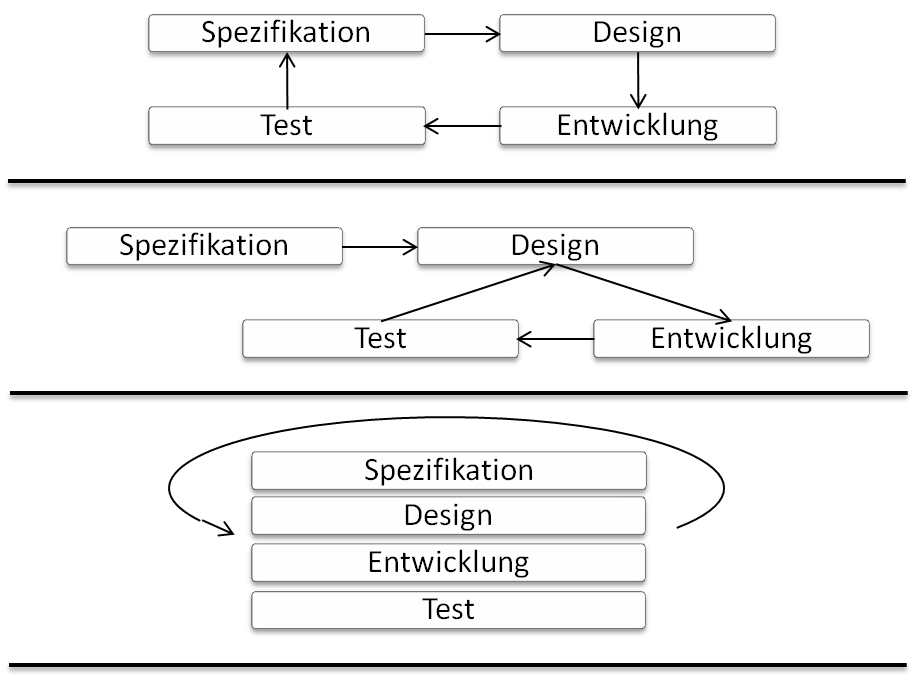
\includegraphics[scale=0.8]{img/iterativeentwicklungsmodelle.png}\\
  \footnotesize\sffamily\textbf{Quelle:} \cite[vgl. S.24]{seidl_basiswissen_2012}
  \caption{Verschiedene Ausprägungen iterativer und agiler Entwicklungsmodelle}
  \label{fig:verschiedene_auspraegungen_iterativer_und_agiler_entwicklungsmodelle}
\end{figure}
Für das Testen stellen diese kurzen Iterationen laut  Seidl et al. \cite[vgl. S.24]{seidl_basiswissen_2012} ein Problem dar.
Jeder Entwicklungszyklus bringt neue Features hervor, die mit Testfällen abgedeckt werden müssen. Der agile Charakter in diesen Vorgehensmodellen bedingt, dass sich Anforderungen ständig ändern und somit auch bereits fertiger Code oft angepasst werden muss. Darüber hinaus ist nicht ausgeschlossen, dass neue Features Auswirkungen auf alten Code haben können. Neben den neu implementierten Teilen muss daher zum Ende einer jeden Iteration auch sämtlicher alter Code getestet werden.
Dies bedingt einen enormen zusätzlichen Testaufwand. 
In agilen Vorgehensmodellen, wie Scrum, ist der Testaufwand nach wenigen Sprints bereits oft so hoch, dass ein Testdurchlauf zusammen mit allen Regressionstests manuell nicht mehr zu bewältigen ist.
Gerade in Projekten, die einem derartigen Vorgehensmodell folgen, ist es daher sinnvoll Testautomatisierung einzusetzen. Einmal implementierte Testfälle können zum Ende einer jeden Iteration erneut ausgeführt werden. Die höheren Kosten, die bei der Automatisierung entstehen, sind so schnell amortisiert.\\
Das sich ständig ändernde Testobjekt bedingt nicht nur die Notwendigkeit von automatisierten Testfällen, sondern erhöht gleichzeitig auch die Anforderungen an die Qualität. Häufige Änderungen am zu testenden Code lassen einmal implementierte Testfälle schnell veralten. Es muss daher bei der Erstellung der automatisierten Tests besonders auf die Wartbarkeit geachtet werden.
Testfälle sollten möglichst robust in ihrem Design sein, um nicht schon bei kleinen Änderungen zerstört zu werden. Der Qualitätsstandard sollte den gleichen Anforderungen unterliegen, der bereits für den vorhandenen Code verwendet wurde. Anpassungen werden sonst zu zeitaufwendig. Die Pflege der bereits implementierten Testfälle ist dann nicht mehr wirtschaftlich und die Akzeptanz der Tests im Projekt sinkt.

\newpage
\chapter{Testautomatisierung}
\label{sec:testautomatisierung}


\section{Warum Testautomatisierung}
\label{sec:warum_testautomatisierung}



\section{Bereiche der Testautomatisierung}
\label{sec:bereiche_der_estautomatisierung}
Einteilung nach testprozess nicht perfekt. Dahre eine einteilung die der automatisierung besser passt:
A Search-Based Approach for Cost-Effective Software Test Automation Decision Support and an Industrial Case Study

\subsection{Testdesign}
\label{subsec:testdesign}


\subsection{Testcodeerstellung}
\label{subsec:testcodeerstellung}
c&r

\subsection{Testdurchführung}
\label{subsec:testdurchführung}


\subsection{Testauswertung}
\label{subsec:testauswertung}



\section{Schnittstellen der Testautomatisierung zum System}
\label{sec:schnittstellen_der_testautomatisierung_zum_syste}

Jeder testfall muss in irgendeiner weise mit dem zu testenden objekt interagieren.
Analog zu manuellen tests gibt es hierfür verschiedene möglichkeiten.
\subsection{API}
\subsubsection{JUnit}
\label{sec:junit}

\subsection{GUI}
Web

\newpage
\chapter{Testautomatisierung mit Selenium}
\label{sec:testautomatisierung_mit_selenium}

Laut Seidel et al. \cite[vgl. S. 48]{seidl_basiswissen_2012} ist der am meisten verbreitete \frqq Angriffspunkt\flqq\ für Testautomatisierung die grafische Benutzerschnittstelle. Seidel et al. \cite[S. 48]{seidl_basiswissen_2012} nennen dafür folgende Gründe:
\begin{itemize}
\item \glqq Sie ist für Tester und Automatisierer anschaulich und leicht greifbar.\grqq
\item \glqq Sie stellt zumeist das Verhalten im realen Umfeld am besten nach.\grqq
\item \glqq Die Dokumentation von Systemen ist auf dieser Ebene meist am vollständigsten.\grqq
\item \glqq Der klassische Systemtest wird oft über diese Schnittstelle abgewickelt.\grqq
\item \glqq Hinter der grafischen Benutzerschnittstelle liegende Systeme werden implizit getestet.\grqq
\end{itemize}
Ein großer Teil der heutzutage entwickelten Anwendungen werden in Form einer Webapplikation realisiert. Im Bereich der Testautomatisierung die als Schnittstelle die grafische Benutzeroberfläche verwenden, stellen diese Webapplikation einen Sonderfall dar.
Im Gegensatz zu gewöhnlichen Denktopanwendungen gibt es bei dieser Art von Anwendung laut Seidel et al. \cite[vgl. S. 88]{seidl_basiswissen_2012} \glqq keinen spezifischen Client für eine Applikation, sondern einen generischen - den Browser.\grqq\ Dies schafft nach Seidel et al.  \cite[vgl. S. 59]{seidl_basiswissen_2012} \glqq für Werkzeuge eine sehr gute Basis, um auf die Elemente der Seite zuzugreigen.\grqq\ Die einzelnen HTML-Elemente und deren Attribute können verwendet werden um die Bestandteile eine Seite zu adressieren.
Ein weit verbreitetes Tool für die Automatisierung, welches diesen Ansatz verfolgt ist Selenium \cite{selenium_selenium_2015}.
\section{Selenium}
\label{sec:selenium}
Seidel et al. \cite[S. 142]{seidl_basiswissen_2012} beschreiben Selenium als \glqq eines der gängigsten Open-Source-Automatisierungswerkzeuge für Webapplikationen.\grqq\
Ordnet man Selenium der in Kapitel \ref{subsec:testcodeerstellung} gewählt Unterteilung der Testautomatisierung zu, befindet sich Selenium im unteren mittleren und unteren linken Quadranten. Abbildung \ref{fig:bereicheTestcodeerstellungSelenium} hinterlegt diese Bereiche farblich.
Selenium ist also ein Tool mit welchem Testfälle erstellt werden können die als Schnittstelle die grafische Benutzeroberfläche eine Webanwendung verwenden. Die Testfälle können dabei manuell programmiert oder über einen \grq record-and playback\grq -Mechanismus aufgezeichnet werden.
\begin{figure}[htb]
  \centering  
  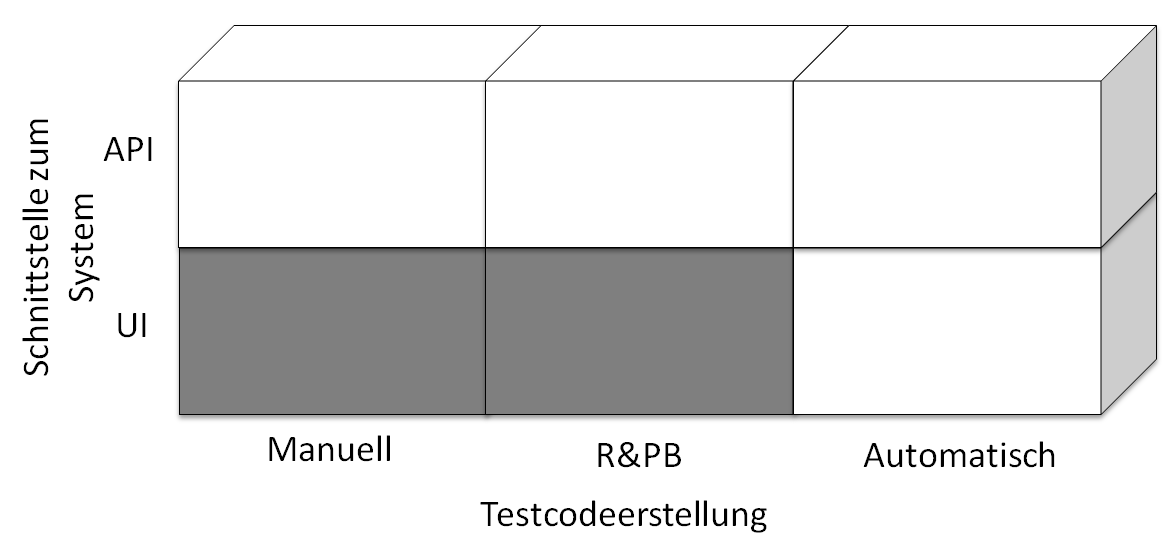
\includegraphics[scale=0.7]{img/bereicheTestcodeerstellungSelenium.png}\\
  \footnotesize\sffamily\textbf{Quelle:} vgl. \cite{meszaros_agile_2003}
  \caption{Einordnung von Selenium in die verschiedene Möglichkeiten der Testcodeerstellung}
  \label{fig:bereicheTestcodeerstellungSelenium}
\end{figure}
Genau genommen handelt es sich bei Selenium aber nicht um ein einzelnes Tool, sondern um eine Reihe von Tools die unter dem Namen Selenium zusammengefasst werden.
In seiner aktuellen Ausprägung 2.x lassen sich, abgesehen von Komponenten die der Abwärtskompatibilität dienen, laut Dokumentation \cite{selenium_selenium_2015-1} drei Komponenten unterscheiden:

\begin{itemize}
\item Selenium IDE \\
Bei der Selenium IDE handelt es sich um ein Firefox plug-in, das verwendet werden kann um Selenium-Testscripte zu erstellen. Testscripte können dabei von Hand erstellt oder mittels eines \grq record-and playback\grq -Mechanismus direkt im Browser aufgezeichnet werden. Die erstellten Testfälle können mit Akzeptanzkriterien angereichert werden und innerhalb der IDE wieder abgespielt werden.
\item Selenium WebDriver \\
Der Selenium WebDriver bietet für verschiedene Programmiersprachen eine API zur Steuerung eines Browsers aus dem Programmcode heraus. Der WebDriver bildet damit die Kernkomponente für alle Selenium-Testfälle die außerhalb der Selenium IDE entwickelt werden.

\item Selenium Server/Grid \\
Mit Hilfe des Selenium Servers ist es möglich Selenium-Testfälle nicht nur auf dem eigenen Rechner auszuführen sondern die Ausführung auf einen Server auszulagern. Einen wichtigen Teil des Selenium Server bildet Selenium Grid. Selenium Grid bietet die Möglichkeit die Ausführung von Selenium-Testfällen über einen Server hinaus auf eine Vielzahl von Knoten zu verteilen. Selenium Server dient dann als Hub der die Testfallanfragen auf Registriert Knoten zur Ausführung weiterleitet. 
\end{itemize}


\section{Testdurchführung mit Selenium}
\label{sec:testdurchführung_mit_selenium}
Abhängig davon ob die Testfälle für die Selenium IDE entwickelt wurden oder sich auf den Selenium WebDriver stützen unterscheiden sich die Möglichkeiten zur Ausführung der Testskripte.\\
Testfälle die mit der Selenium IDE entwickelt wurden verwenden eine Selenium eigene Sprache mit dem Namen \grq Selense\grq.\ Diese Testfälle können in späteren Testläufen wieder über die Selenium IDE zur Ausführung gebracht werden. \\
Dem gegenüber stehen Testfälle die den Selenium WebDriver verwenden.
Testfälle die mittels Selenium WebDriver entwickelt wurden sind für ihre Ausführung nicht an ein spezielles Tool gebunden. Beim WebDriver handelt es sich um eine API mit deren Hilfe ein Browser ferngesteuert werden kann. Wie diese API in die Testfälle integriert wird ist dem Entwickler selbst überlassen. In der Praxis hat sich als Best Practice jedoch herausgestellt, dass Selenium-Testfälle, die den WebDriver verwenden, meist in Verbindung mit einem Unit Testing Framework entwickelt werden.
Im Java Umfeld wären hier beispielsweise JUnit oder TestNG zu nennen.
Die Testfälle können damit analog zu den klassischen Unit Tests entwickelt werden, verwenden jedoch als Schnittstelle zum System nicht die API sondern, über den WebDriver, die Benutzeroberfläche. 
Die Ausführung der Testfälle erfolgt dann analog zu den klassischen Unit Tests über das Unit Testing Framework.
Im Bereich des WebDrivers stützt sich Selenium also auf bereits sehr gut etablierte Frameworks. Das hat den Vorteil, dass die so erstellten Testfälle bereits in den meisten Programmiersprachen gut in die Infrastruktur integriert sind. In Java sind Testfälle die mittels JUnit ausgeführt werden in allen gängigen IDEs durch Plugins unterstützt. Noch viel wichtiger ist jedoch eine gute Integration der Testfälle in den Buildprozess. Werden beispielsweise in Java Standarttools wie Gradle oder Maven zum bauen der Projekte verwendet, können die Testfälle ohne Mehraufwand im Rahmen des Buildprozesses ausgeführt werden.



\section{Testcodeerstellung mit Selenium}
\label{sec:Testdesign}
Die Testcodeerstellung von Testfällen die Selenium verwenden kann auf zwei Arten erfolgen.
Testcode kann Manuell erstellt werden oder über einen \grq record-and playback\grq -Mechanismus teilautomatisiert generiert werden.

\subsection{Recorde-and-playback}
\label{sec:recorde_and_playback}
Die Selenium IDE bietet die Möglichkeit Testskripte mittels \grq record and playback\grq\ zu erzeugen.
Die im Testfall gewünschten Abläufe können dabei einfach im Browser abgearbeitet werden.
Die durchgeführten Schritte werden von der Selenium IDE in der Selenium eigenen Sprache \grq Selense\grq\ aufgezeichnet. Diese Aufzeichnungen können später von der Selenium IDE interpretiert werden um so die Testabläufe erneut zu wiederholt.
Testskripte können nach dem Aufzeichnen nachträglich überarbeitet werden. Damit können beispielsweise Akzeptanzkriterien an bestimmten Stellen im Testablauf eingearbeitet werden.\\
Testfälle die über den \grq record-and playback\grq -Mechanismus erstellt wurden sind nicht an die Sprache \grq Selense\grq\ gebunden. Die Selenium IDE bietet die Möglichkeit die Testskripte in eine Reihe von Programmiersprachen zu exportieren. Darunter beispielsweise auch Java.
Diese Testfälle benutzen dann wie in Abschnitt \ref{sec:testdurchführung_mit_selenium} beschrieben, den Selenium Webdriver für die Kommunikation mit dem Browser und ein Unit Testing Framework für die Ausführung.\\
Die \grq record and playback\grq -Funktionalität bietet eine besonders einfache und schnelle Möglichkeit um Testfälle zu erstellen. Dennoch wird in der Dokumentation von Selenium \cite{selenium_selenium_2015-1} davon abgeraten sich bei der Testfallerstellung alleine auf dieses Tool zu stützen. Die Selenium IDE wird als Prototyping-Tool verstanden mit dem kleine Aufgaben, die nicht für den längerfristigen Einsatz gedacht sind, schnell automatisiert werden können.
Testabläufe die über den \grq record-and playback\grq -Mechanismus in der IDE erstellt werden unterliegen eine Reihe von Limitierungen. Leotta et al. \cite{leotta_repairing_2013} nennen als Limitierungen dieser Testfälle das fehlen von bedingten Anweisungen, Schleifen, Logging, Ausnahmebehandlungen so wie parametrisierten (a.k.a. data-driven) Testfällen.
Neben diesen Limitierungen haben die Testfälle zusätzlich das Problem, dass sie eine schlechte Wartbarkeit aufweisen. Nach Leotta et al. \cite{leotta_repairing_2013} liegt das vor allem daran, dass die Testfälle sehr stark mit der Struktur der Webseiten verwoben sind und einen hohen Anteil an dupliziertem Code aufweisen.
Die Limitierungen der IDE können zwar durch das Exportieren der Testfälle in eine Programmiersprache überwunden werden, die Qualität der Testfälle im Bezug auf ihre spätere Wartbarkeit kann nach  Leotta et al. \cite{leotta_repairing_2013} auf diesem Wege jedoch nicht verbessert werden.\\
Um die starke Verwobenheit mit der Webanwendung und den hohen Anteil an dupliziertem Code zu veranschaulichen wurden zwei Testfälle über den \grq record-and playback\grq -Mechanismus von Selenium erstellt und in die Programmiersprache Java exportiert.
Die Beiden Testfälle sollen das anlegen und editieren eines Datensatzes auf einer einfachen Web-Anwendung überprüfen.
Drei Seiten der Webanwendung werden für diesen Testfall verwendet. Die Seiten sind in Abbildung \ref{fig:toDoApp} dargestellt.

\begin{figure}[htb]

 \subfigure[Anlegen eines neuen Datensatzes]{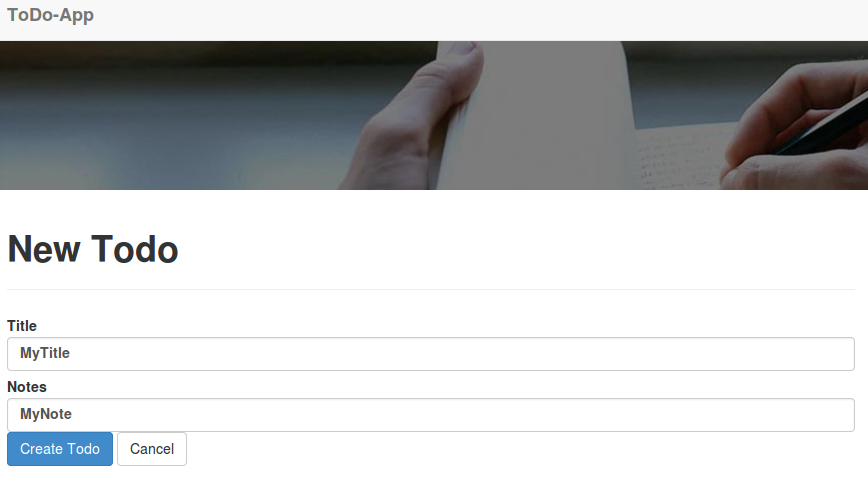
\includegraphics[width=0.49\textwidth]{img/newTodo.png}}
  \subfigure[Anzeigen eines Datensatzes]{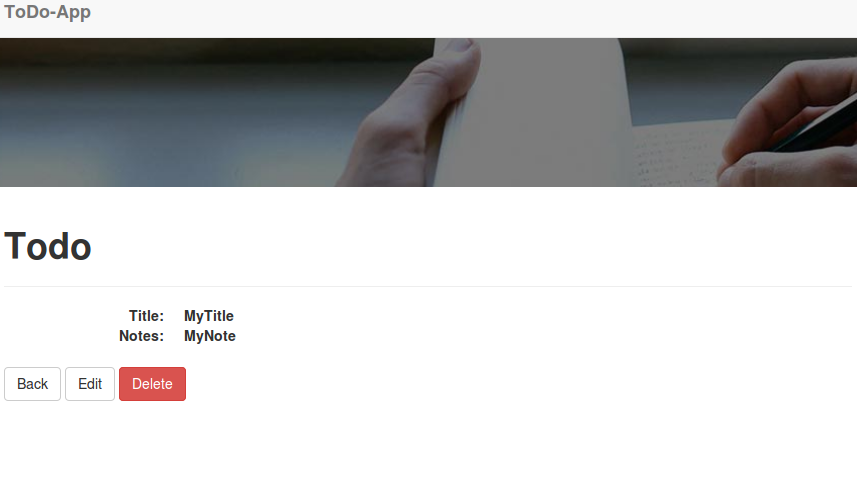
\includegraphics[width=0.49\textwidth]{img/showTodo.png}}
 \subfigure[Editieren eines Datensatzes]{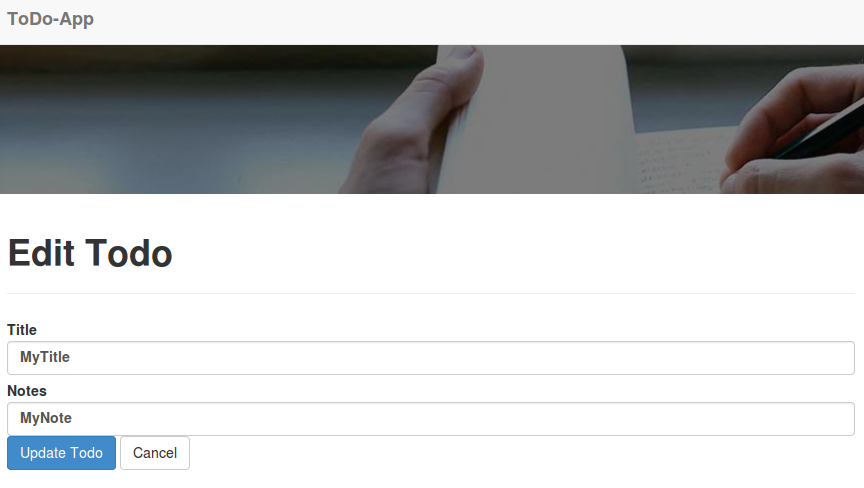
\includegraphics[width=0.49\textwidth]{img/editTodo.png}}
 \caption{Anlegen, Editieren und Anzeigen eines neuen Datensatzes}
  \label{fig:toDoApp}
\end{figure}


Zur besseren Lesbarkeit wurden die Testfälle im Listing \ref{lst:exportierteTestfaelle} leicht überarbeitet, in ihrem Wesen jedoch nicht verändert.
\begin{lstlisting}[caption={Exportierte Testfälle},label={lst:exportierteTestfaelle}]
  /**
  * Testfall legt einen neuen Datensatz an.
  */
  @Test
  public void testCreateNewRecord() {
    WebDriver driver = new FirefoxDriver();
    driver.get("http://localhost:3000/todos/new");
    driver.findElement(By.id("todo_title")).sendKeys("MyTitle");
    driver.findElement(By.id("todo_notes")).sendKeys("MyNote");
    driver.findElement(By.name("commit")).click();
  
    assertEquals("MyTitle", driver.findElement(By.id("title")).getText());
    assertEquals("MyNote", driver.findElement(By.id("note")).getText());
  }
  
  /**
  * Testfall legt einen neuen Datensatz an und editiert ihn.
  */
  @Test
  public void testEditRecord() {
    WebDriver driver = new FirefoxDriver();
    driver.get("http://localhost:3000/todos/new");
    driver.findElement(By.id("todo_title")).sendKeys("MyTitle");
    driver.findElement(By.id("todo_notes")).sendKeys("MyNote");
    driver.findElement(By.name("commit")).click();
    driver.findElement(By.linkText("Edit")).click();
    driver.findElement(By.id("todo_title")).clear();
    driver.findElement(By.id("todo_title")).sendKeys("MyTitleEdit");
    driver.findElement(By.id("todo_notes")).clear();
    driver.findElement(By.id("todo_notes")).sendKeys("MyNoteEdit");
    driver.findElement(By.name("commit")).click();
    
    assertEquals("MyTitleEdit", driver.findElement(By.id("title")).getText());
    assertEquals("MyNoteEdit", driver.findElement(By.id("note")).getText());
  }
  
\end{lstlisting}
Die Testfälle für das Anlegen und Editieren sind in ihren Abläufen recht ähnlich. Beide Testfälle legen zunächst einen neuen Datensatz in der Anwendung an. Die Logik die hierfür verwendet wird ist in beiden Testfällen dupliziert worden. Das ist nicht nur ein Problem dieses Beispiels sondern ein Problem, dass durchaus hohe Praxisrelevanz hat. In den meisten Testabläufen finden sich wiederkehrende Aufgaben, wie beispielsweise einen Login, der nicht nur von einem Testfall benötigt wird.
Selbst wenn sich die Abläufe zwischen den Testfällen stark unterscheiden werden Elemente, z.B. Input-Felder, die von der Anwendung angeboten werden in der Regel nicht nur einmal benutzt. Das führt zwangsläufig dazu, dass die Logik zum adressieren dieser Felder in einer Vielzahl von Testfällen dupliziert wird.\\
Die Adressierung der Elemente in der Anwendung bedingt auch die hohe Koppelung der im Listing \ref{lst:exportierteTestfaelle} gezeigten Testfälle mit den Seiten der Anwendung die Leotta et al. \cite{leotta_repairing_2013} als weiters problem identifiziert haben. Die Selektoren die verwendet werden um die Elemente der Webanwendung anzusteuern sind direkt in den Testfall eingearbeitet. Änderungen an der Seitenstruktur der Anwendung haben damit direkten Einfluss auf die Testfälle.\\
Obwohl sich die eigentliche Testfallspezifikation durch eine Änderung in der Seitenstruktur nicht ändert, müssen die Testfälle trotzdem überarbeitet werden.
Der duplizierter Code und der hohe Grad an Koppelung mit der Anwendung innerhalb der Testfälle bedingen, dass selbst kleine Änderungen in der zu testenden Anwendung, Korrekturen an vielen Stellen in den Testfällen nötig machen.

\subsection{Manuell}
\label{sec:manuell}
Eine weitere Möglichkeit bildet das manuelle Erstellen der Testskripte. Für die Ausführung und die Kommunikation mit der Anwendung verwenden die manuell erstellten Skripte das selbe Toolset wie die generierten und exportierten Testfälle aus der \grq record-and playback\grq -Variante. Analog zu den in Listing \ref{lst:exportierteTestfaelle} gezeigten Testfällen wird der Selenium WebDriver für die Kommunikation mit der Anwendung verwendet. Die Ausführung geschieht über ein Unit Testing Fraemwork.
Im Vergleich zu den halbautomatisch generierten Testfällen ist das manuelle entwickeln der Testskripte aufwändiger.
Es bietet jedoch die Möglichkeit die in Abschnitt \ref{sec:recorde_and_playback} genannten Problemen der \grq record-and playback\grq -Variante entgegenzuwirken.
Bei einem manuellen Ansatz kann von Anfang an auf eine wartbare und wiederverwertbare Struktur in den Testfällen geachtet werden.
Als best practice hat sich zu diesem Zwecke das Page Object Design Pattern durchgesetzt.

\subsection{Page Object Pattern}
\label{sec:page_object_pattern}
Im Page Object Pattern wird versucht die Funktionalität welche die zu testende Anwendung anbietet in einem objektorientierten Ansatz zu kapseln.
Alle Seiten der zu testenden Anwendung werden dazu als Objekte Modelliert. Auf diese Weise wird die Funktionalität die von einer Seite angeboten wird zu einem Service, beispielsweise einer Methode, die von dem korrespondierendem Page Object angeboten werden.
Alle Informationen und Funktionalität die von einer Seite angeboten werden sind so zentral gekapselt.
Ein Page Objekt ist also eine objektorientierte Klasse die als Interface für eine Seite der zu testenden Anwendung dient.
Sämtliche Interaktion mit der zu testenden Anwendung geschieht über die in den Page Objekten angeboten Schnittstellen.
Änderungen an der Oberfläche der zu testenden Anwendung haben so keinen direkten Einfluss mehr auf die Testfälle. Bei Änderungen an der Benutzeroberfläche muss nur noch Code an einer Stelle innerhalb der Page Objekte angepasst werden.\\
Um das Zusammenspiel zwischen Page Objekten und Testfall besser zu verdeutlichen wurde der Testfall zum anlegen eines neuen Eintrags aus Listing \ref{lst:exportierteTestfaelle} im Page Object Pattern nachgebaut.

Der Testfall Arbeitet mit zwei Seiten der Anwendung. Die Seiten sind in Abbildung \ref{fig:toDoApp} dargestellt. Für jede der beiden Seiten wird ein Page Object als Kommunikationsschnittstelle benötigt. 
Das Page Object CreatPage in Listing \ref{lst:poCreatePage} repräsentiert die Seite zum anlegen eines neuen Datensatzes (Abbildung \ref{fig:toDoApp} a). Das Page Object ShowPage in Listing \ref{lst:poShowPage} repräsentiert die Seite zum anzeigen eines Datensatzes (Abbildung \ref{fig:toDoApp} b).

\begin{lstlisting}[caption={Page Object CreatePage},label={lst:poCreatePage}]
  public class CreatePage extends BasePo {
		public final Control tfTodotitle = control(by.textField("todo_title"));
		public final Control tfTodonotes = control(by.textField("todo_notes"));
		public final Control bCreateTodo = control(by.button("commit"));

		public CreatePag(PageObject po) {
			super(po);
		}
		public ShowPage createEntry(String title, String note){
			tfTodotitle.sendKeys(title);
			tfTodonotes.sendKeys(note);
			bCreateTodo.click();
			return new ShowPage(this);
		}
  }
\end{lstlisting}  
\begin{lstlisting}[caption={Page Object ShowPage},label={lst:poShowPage}]  
  public class ShowPage extends BasePo {
		public final Control idTitle = control(by.id("title"));
		public final Control idNotes = control(by.id("note"));

		public ShowPage(PageObject po) {
			super(po);
		}
  }
\end{lstlisting}

Die Funktionalitäten die von den jeweiligen Seiten angeboten werden sind innerhalb des Page Objects gekapselt. Das Page Object CreatPage bietet beispielsweise die Eingabefelder für Titel und Note so wie den Button zum anlegen eines Datensatzes als globale Objekte von Typ Control an.
Die Klasse Control dient in den dargestellten Page Objekten als Wrapper für den Selenium WebDriver. Control-Objekte sind also analog zu Selenium WebElementen zu verstehen.
Die Funktionalität zum anlegen eines neuen Eintrags die im späteren Testfall benötigt wird bietet das Page Objekt CreatPage als Service-Methode \grq createEnty()\grq\ an.\\

Der Testfall in Listing \ref{lst:pageObjectTestfall} verwendet die Beiden Page Objekte um einen neuen Eintrag in der Anwendung anzulegen und zu überprüfen.


\begin{lstlisting}[caption={Page Object Testfall},label={lst:pageObjectTestfall}]  
  /**
  * Testfall legt einen neuen Datensatz an.
  */
 	@Test
	public void testCreateNewRecord(){
		CreatePage createPage = new CreatePage(po);
		ShowPage showPage = createPage.createEntry("MyTitle", "MyNote");

		assertEquals("MyTitle", showPage.idTitle.resolve().getText());
		assertEquals("MyNote", showPage.idNotes.resolve().getText());
	}

\end{lstlisting}

Im Gegensatz zum Testfall in Listing \ref{lst:exportierteTestfaelle} ist es auf Grund des Page Object Pattern nicht mehr nötig explizite Referenzen auf die Struktur der Seite innerhalb der Testfälle zu machen. Alle Details der Seite sind innerhalb der PageObjekte gekapselt. Der Testfall verwendet lediglich die im Page Object angebotenen Funktionalität.


\subsubsection{Vorteile des Page Object Pattern}
\label{sec:vorteile_des_page_object_pattern}

Folgende Vorteile ergeben sich damit bei der Verwendung des Page Object Pattern die auch so in der Selenium Dokumentation \cite{selenium_selenium_2015-2} angegeben werden:

\begin{enumerate}
\item Es gibt eine klare Trennung zwischen Testcode und seitenspezifischem Code wie beispielsweise Elementadressierungen und Layout. \\ \\
Die Adressierung der Elemente ist nicht mehr über die gesamten Testfälle verteilt sondern befindet sich an einem zentralen Ort, dem Page Object.
Die hohe Koppelung der Testfälle mit den Seiten der Anwendung die Leotta et al. \cite{leotta_repairing_2013} als Problem genannt haben kann somit überwunden werden.

\item Es gibt einen einzigen Ort für die Elemente und Operationen die von einer Seite angeboten werden. \\ \\
Alle Informationen die eine Seite der Anwendung betreffen sind an einem zentralem Ort, dem Page Object gesammelt. Seitenspezifischer Code muss somit nicht mehr in den einzelnen Testfällen dupliziert werden. Die Funktionalitäten der Seite können über das entsprechende Page Object abgerufen werden.

\end{enumerate}

Beide Vorteile führen dazu, dass Änderungen die an einer Seite gemacht werden nur Auswirkungen an einem zentralen Stelle haben. Die Wartbarkeit der gesamten Testfälle wird so erhöht.
Leotta et al. unterstützen diese These mit einer Fallstudie \cite{leotta_repairing_2013} in der Sie eine herkömmliche Testsuite mit einer Testsuite die das Page Object Pattern implementiert hinsichtlich ihrer Wartbarkeit verglichen haben.
Das Ergebnis dieser Studie hat gezeigt, dass in Ihrem Fall die Zeit für die Wartung der Testfälle um ca. 65\% reduziert werden konnten. Die Anzahl der anzupassenden Codezeilen konnte um ca. 87\% reduziert werden.

\subsubsection{Probleme des Page Object Pattern}
\label{sec:probleme_des_page_object_pattern}

Die Vorteile des Page Object Pattern kommen allerdings mit einem Preis. Die Komplexität des gesamten Testprojekts steigt. Testfälle können nicht mehr beliebig programmiert werden sondern sind in den Kontext von Page Objekts zu stellen. Das erfordert tiefgründige Designentscheidungen. So ist beispielsweise zu klären wie über die Page Objekts ein generischer Einstieg in die Anwendung angeboten werden kann oder wie der WebDriver über mehrere Page Objekts und Testfälle hinweg verwaltet werden kann. Auch die Page Objects selbst müssen erst einmal entwickelt werden bevor mit dem erstellen von Testfällen begonnen werden kann.\\
Verglichen mit einem herkömmlichen Ansatz steigt mit der Verwendung des Page Object Pattern zu Beginn also der Aufwand beim erstellen eines Testprojektes. Leotta et al. \cite{leotta_repairing_2013} haben gezeigt, dass sich diese Investition durchaus lohnen kann, initial sind die Kosten allerdings höher.

\newpage

\chapter{Teilautomatisierte Generierung von Page Objects}
\label{sec:teilautomatisierte_generierung_von_pageObjects}

Ein großer Teil des in Kapitel \ref{sec:probleme_des_page_object_pattern} angesprochenen initialen Mehraufwands, bei der Verwendung des Page Object Pattern beläuft sich auf die Erstellung der Page Objects.
Wie in Listing \ref{lst:poCreatePage} und \ref{lst:poShowPage} zu sehen ist, handelt es sich bei Page Objects um weniger komplexe Klassen. In der Praxis zeigt sich, dass ein Großteil der Arbeit darin besteht, die verschiedenen Lokatoren der Elemente aus dem Quelltext der Seite zu extrahieren und in die generische Form eines Page Objects zu überführen.
Diese Aufgabe kostet zwar viel Zeit, ist allerdings nicht sehr anspruchsvoll.
Möchte man den initialen Mehraufwand bei der Verwendung des Page Object Pattern entgegenwirken, liefern die Page Objects somit einen guten Ansatzpunkt.
Aufgrund ihrer generischen Natur bieten sie gute Voraussetzungen, um automatisch generiert zu werden.
\section{Übersicht über die Idee}
\label{sec:uebersicht_ueber_idee}


Selenium, in Verbindung mit dem Page Object Pattern, ist auch ein Teil des Technologiestacks des IT-Dienstleisters (it@M) der Landeshauptstadt München und wird dort zum Testen komplexer Webanwendungen verwendet. Auch it@M hat in Bezug auf die Erstellung von Page Objects die Erfahrung gemacht, dass es sich um eine generische und zeitaufwendige Arbeit handelt.
In Zusammenarbeit wurde daher die Idee entwickelt, das Erstellen von Page Objects mit Hilfe einer Softwarelösung zu unterstützen.
Anhand des Seitenquelltextes der zu testenden Webanwendung sollen die verschiedenen Elemente des Page Objects identifiziert und zur Generierung der Klassen verwendet werden.
Zwei Ansätze wurden dabei diskutiert. Eine vollautomatisierte und eine teilautomatisierte Generierung von Page Objects.\\
Ein vollautomatischer Ansatz würde beinhalten, dass ohne weiteres Zutun aus dem Seitenquelltext ein vollständiges Page Object generiert wird. Dieser Ansatz hat jedoch mit zahlreichen Problemen zu kämpfen. Oft wird nur ein Bruchteil der Elemente einer Webseite für die Testfälle benötigt. Selenium kann aber prinzipiell jedes Element, dass im Seitenquelltext bereitgestellt wird, ansprechen. Bei einer vollautomatischen Generierung müssten daher entweder alle Elemente einer Seite übernommen, oder eine definierte Auswahl getroffen werden.
Wird eine Auswahl getroffen, besteht das Risiko, dass Elemente ausgelassen werden, die vom Tester möglicherweise benötigt werden. Werden alle Elemente übernommen, werden die Page Objects schnell überfüllt und unübersichtlich. Das Überfüllen der Page Objects geschieht dann auf Kosten ihrer Robustheit. Strukturelle Änderungen in der Website wirken sich auch auf die Lokatoren der Elemente aus. Um die Page Objects stabil zu halten, müssen diese bei Änderungen in der Seitenstruktur berichtigt werden.
Es ist daher nicht sinnvoll, Elemente in den Page Objects zu pflegen, die nicht verwendet werden. Unbenutzte Elemente bedeuten entweder zusätzlichen Wartungsaufwand oder veralten unbemerkt.\\
Ein weiteres Problem des vollautomatischen Ansatzes stellen die Übergänge zwischen den Seiten einer Webanwendung dar. Interaktionen, wie beispielsweise das Betätigen eines Links oder Button, führen oft zum Aufrufen einer neuen Seite der zu testenden Webanwendung. Im weiteren werden diese Übergänge als Transitionen bezeichnet. Diese Transitionen werden auch in den Page Objects abgebildet. Das Page Object gibt dazu das entsprechende Page Object der Zielseite als Rückgabe eines Methodenaufrufs der Ausgangsseite zurück. In der Methode \grq CreatePage.createEntry()\grq\ im Listing \ref{lst:poCreatePage} ist diese Vorgehen dargestellt. Allein aus dem Seitenquelltext zu ermitteln, welche Seite das Ziel einer Transition ist, erweist sich oft als sehr schwierig bis unmöglich.\\
Um die Komplexität des Projektes aufgrund der genannten Probleme nicht zu groß werden zu lassen, entschied man sich für eine teilautomatisierte Lösung.
Ziel ist es also nicht, ein vollständiges Page Object vollautomatisiert zu generieren, sondern den Entwickler bei der Generierung der Page Objects zu unterstützen. Anhand des Quelltextes sollen dem Entwickler die möglichen Elemente der Seite in einer Vorauswahl bereitgestellt werden. Aus diesen Elementen können dann diejenigen ausgewählt werden, die im späteren Page Object benötigt werden. Auf diese Weise wird ein Überladen verhindert und gleichzeitig sichergestellt, dass die Elemente, die benötigt werden, vorhanden sind.
Ob es sich bei einem Element um eine Transition handelt, also ein Element, welches auf eine neue Seite führt, muss nicht mehr automatisch anhand des Quelltextes ermittelt werden, sondern wird vom Entwickler direkt bei der Auswahl der benötigten Elemente mit angegeben.
Die so vom Entwickler ausgewählten Informationen können später verwendet werden, um daraus das fertige Page Object zu generieren.
Im Rahmen des Projektes \grq SeleniPo\grq\ soll dieser Ansatz in Zusammenarbeit mit it@M in Form einer Desktopanwendung umgesetzt werden. 

\section{Abgrenzung zu bestehenden Ansätzen}
\label{sec:abgrenzung_zu_bestehenden_ansaetzen}
Sowohl für die vollautomatische Generierung von Page Objects, als auch für eine teilautomatisierte Generierung, gibt es bereits mögliche Lösungsansätze. 
Stocco et al. \cite{stocco_why_2015} beschreiben in einem Paper das von ihnen entwickelte Framework APOGEN, mit deren Hilfe Page Objects vollautomatisch generiert werden können. Die Generierung geht dabei weit über das Anlegen von Elementen hinaus und schließt auch die Funktionalitäten der einzelnen Webseiten in Form von Methoden mit ein.
Das Framework analysiert dazu die Struktur der Webanwendung mittels eines Crawlers. Die Informationen, die über den Crawler zusammengetragen wurden, wie beispielsweise das DOM der einzelnen Webseiten, werden anschließend über eine statische Analyse aufbereitet und für die Generierung der Page Objects verwendet.
Nach Angaben der Forschungsgruppe sollen ca. 75\% des von APOGEN generierten Codes ohne Anpassungen verwendet werden können. Die restlichen 25\% benötigen nur kleine Änderungen.\\
Bei APOGEN handelt es sich jedoch um ein noch sehr junges Projekt. Das entsprechende Paper wurde im Mai 2015 veröffentlicht. APOGEN ist daher eher ein Prototyp, der zwar die Möglichkeiten aufzeigt, die in diesem Bereich gegeben sind, jedoch noch nicht für den produktiven Einsatz in einem großen Unternehmen geeignet ist.
Nach eigenen Angaben leidet das Projekt noch unter einigen Einschränkungen. Eine der genannten Einschränkungen ist die Limitierung durch den Crawler.
APOGEN kann nur Webseiten in Page Objects umwandeln, die auch durch den Crawler erreicht werden.
Für einfache Webanwendungen stellt das kein großes Problem dar, für sehr komplexe Anwendungen mit einer ausgeprägten logischen Validierung allerdings schon.
Viele Seiten, die hinter logisch validierten Eingaben liegen, können vom Crawler nicht erreicht werden und stehen somit für die Generierung nicht zur Verfügung.\\
Neben der vollautomatischen Generierung existieren noch eine Reihe von Open-Source-Framworks,
die einen teilautomatisierten Ansatz verfolgen, ähnlich wie es das Projekt SeleniPo erreichen will.
Stocco et al. \cite{stocco_why_2015} nennen in ihrem Paper die drei derzeit wichtigsten Vertreter:

\begin{itemize}
\item \textit{OHMAP} \cite{virtuetech_gmbh_ohmap_2015}: Bei OHMAP handelt es sich um eine Webseite, die es dem Benutzer erlaubt, HTML-Code in eine Textarea zu kopieren. Aus dem übergebenen HTML-Code generiert das Tool eine einfache Java-Klasse, die für jedes gefundene Input-Feld ein WebElement enthält. Die Variablennamen werden dabei aus den HTML-Attributen gebildet. Als Lokator wird ein einfacher XPath-Ausdruck verwendet.
	
\item \textit{SWD Page Recorder} \cite{dmytro_zharii_dzharii/swd-recorder_2015}: Der SWD Page Recorder ermöglicht es dem Benutzer eine beliebige Webanwendung zu starten und das GUI der Anwendung mit einem \grq click\&record\grq-Mechanismus zu inspizieren.
Nach jedem Klick auf das Interface der Anwendung wird ein Dropdown-Menü angezeigt, in welches manuell ein Name für das ausgewählte Element eingetragen werden kann. Als Lokator wird ein einfacher XPath-Ausdruck generiert.
Das so erstellte Modell der Anwendung kann in verschiedene Sprachen exportiert werden, wie beispielsweise Java, C\#, Python, Ruby oder Perl. Beim SWD Page Recorder handelt es sich um eine .NET Anwendung.

\item\textit{ WTF PageObject Utility Chrome Extension} \cite{daniel_wiredrive/wtframework_2015}: WTF unterstützt den Entwickler beim Erstellen von Page Objects, indem Lokatoren der Form id, name, CSS oder XPath erstellt werden. Der Code wird in Python generiert.
	
\end{itemize}

Der Technologiestack von it@M sieht eine Entwicklung der Selenium-Testfälle in Java vor. Als Betriebssystem kommt darüber hinaus Linux zum Einsatz.
Zwei der genannten Lösungsansätze scheiden mit dieser Einschränkung für den produktiven Einsatz beim IT-Dienstleister der Landeshauptstadt München aus. Beim SWD Page Recorder handelt es sich um eine .NET Anwendung, die nur schwer unter Linux betrieben werden kann. Die WTF PageObject Utility Chrome Extension kann nur im Python-Umfeld betrieben werden. OHMAP wäre aus technischer Sicht eine mögliche Lösungsalternative. Allerdings sind Komfort und Umfang der Anwendung aus Sicht von it@M nicht ausreichend. Ohne eigene Konfiguration ist es mit OHMAP nur möglich, input-Felder zu erkennen.
Darüber hinaus muss der HTML-Quelltext händisch aus der zu testenden Anwendung extrahiert werden. \\
Sowohl OHMAP, als auch der SWD Page Recorder haben zusätzlich das Problem, dass die erzeugten XPath Ausdrücke oft sehr einfach gewählt werden und damit sehr stark von der Position der Elemente innerhalb der Seite abhängig sind. Die eigentlichen Charakteristika der Elemente werden oft nicht beachtet. Listing \ref{lst:badXPath}
zeigt einen solche von OHMAP generierten XPath.

\begin{lstlisting}[caption={Einfacher XPath-Lokator des Projektes OHMAP},label={lst:badXPath}]
	public class YourPageObjectName {
		//...		
 		@FindBy(xpath = "/html/body/div/div[1]/div[1]/h1/a[2]")
		public WebElement followVirtuetechGmbH;	
		//...
	}
\end{lstlisting}

Der zu adressierende Link in Listing \ref{lst:badXPath} wird alleine über seine Position innerhalb des DOM der Seite bestimmt.
Um den Lokator zu zerstören würde es genügen, ein weiteres div-Tag vor dem Link einzufügen. Bezieht man den XPath auf die eigentlichen Charakteristika, wie beispielsweise ein id-Attribut, können sehr viel stabilere Ausdrücke erzeugt werden.
\\
Negativ ist an allen gezeigten Lösungen, dass sie immer nur ein Page Object auf einmal betrachten. Transitionen, also Übergänge zwischen den einzelnen Webseiten der zu testenden Anwendung, werden nicht beachtet. Die dynamische Komponente der Anwendung wird beim Generieren der Page Objects außer Acht gelassen und muss nachträglich händisch hinzugefügt werden.

Mit SeleniPo soll der Versuch unternommen werden, die Schwachstellen der bereits existierenden Lösungsansätzen zu verbessern und eine plattformunabhängige Lösung zu schaffen, die in der IT-Infrastruktur von it@M ausgeführt werden kann.

\newpage
\section{SeleniPo - Page Object Generator}
\label{sec:selenipo_pogenerator}

Abbildung \ref{fig:poGenerator} zeigt die Denktopanwendung (Page Object Generator), die im Rahmen des Projektes SeleniPo entwickelt wurde. Mit Hilfe dieser Anwendung können Page Objects teilautomatisiert generiert werden. Es wird dazu die Möglichkeit geboten, einen Browser zu starten und über vorgefertigte Selektoren die Webanwendung nach benötigten Elementen bzw. Transitionen zu durchsuchen. Auf diese Weise kann ein Modell der Anwendung erstellt werden, dass zur Generierung der Page Objects verwendet wird.

\begin{figure}[htb]
  \centering  
  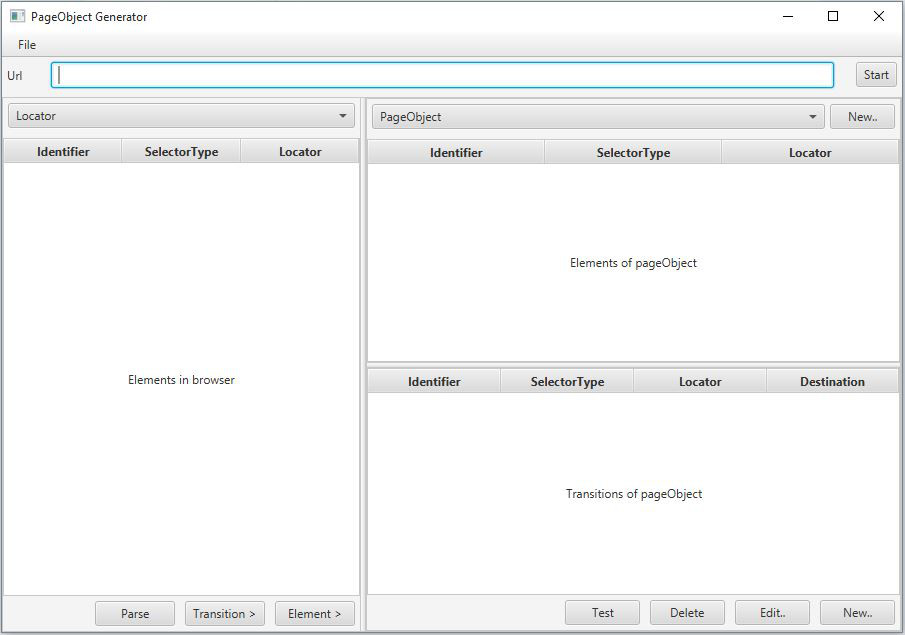
\includegraphics[scale=0.5]{img/poGenerator.JPG}\\
  \caption{SeleniPo - Page Object Generator}
  \label{fig:poGenerator}
\end{figure}



Die Benutzeroberfläche des Page Object Generators teilt sich in drei Bereiche:

\begin{itemize}
	\item Das aktuelle Page Object Modell (Abbildung \ref{fig:poGeneratorPo})
	\item Den HTML-Parser (Abbildung \ref{fig:poGeneratorHtml})
	\item Das Menü (Abbildung \ref{fig:poGeneratorMenu})
\end{itemize}


Abbildung \ref{fig:poGeneratorPo} zeigt den Bereich des Generators, mit dem das aktuelle Page Object Modell der zu testenden Anwendung verwaltet werden kann. Mit diesem Teil der Anwendung können neue Page Objects angelegt und bearbeitet werden. Elemente und Transitionen können manuell hinzugefügt, editiert oder gelöscht werden. Darüber hinaus besteht die die Möglichkeit, existierende Elemente und Transitionen auf ihre Richtigkeit zu testen.

\begin{figure}[htb]
  \centering  
  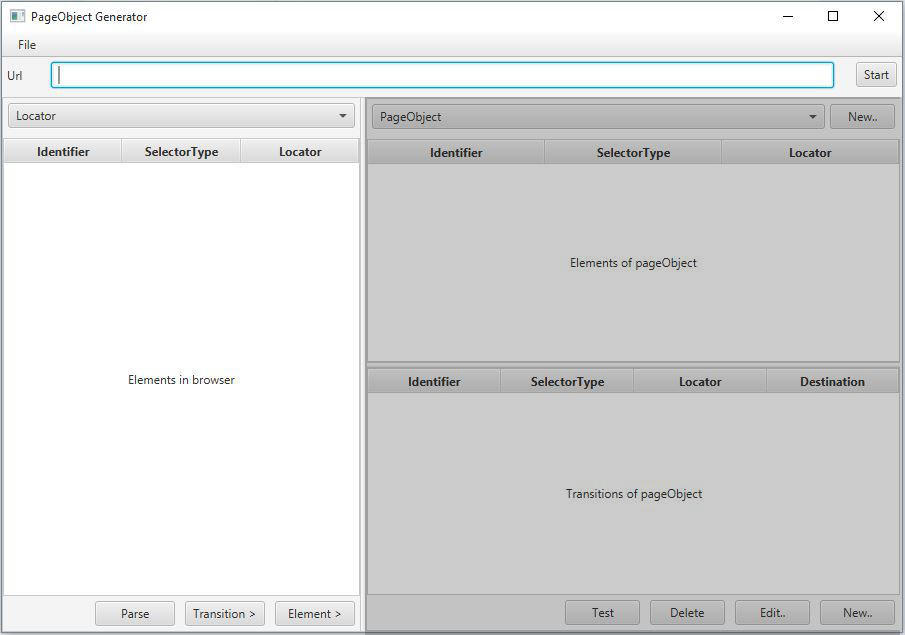
\includegraphics[scale=0.5]{img/poGeneratorPo.JPG}\\
  \caption{SeleniPo - Page Object Generator - Page Object Model}
  \label{fig:poGeneratorPo}
\end{figure}

\newpage

Abbildung \ref{fig:poGeneratorHtml} zeigt den Bereich des Generators, mit dem der Entwickler bei der Erstellung von Elementen und Transitionen im Page Object unterstützt werden kann.
Über den Start-Button kann ein Browser gestartet werden. Über das Lokator-Dropdown kann mittels vorgefertigten Selektoren die aktuell im Browser dargestellte Webseite nach Elementen bzw. Transitionen durchsucht werden. Im Page Object benötigte Elemente und Transitionen können dann in das ausgewählte Page Object übernommen werden, um so ein Page Object Modell der zu testenden Webanwendung zu erstellen.

\begin{figure}[htb]
  \centering  
  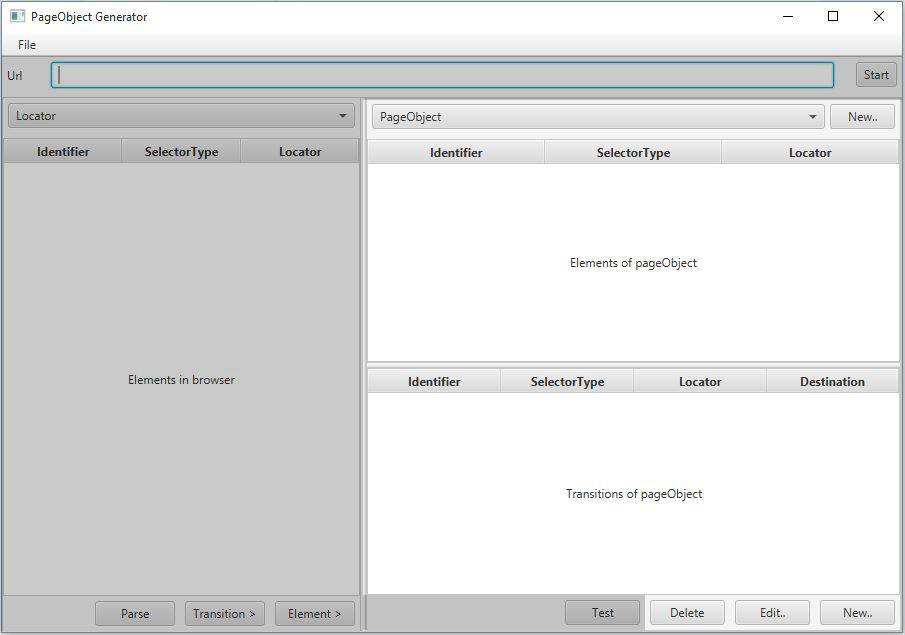
\includegraphics[scale=0.5]{img/poGeneratorHtml.JPG}\\
  \caption{SeleniPo - Page Object Generator - HTML Parser}
  \label{fig:poGeneratorHtml}
\end{figure}

\newpage

Abbildung \ref{fig:poGeneratorMenu} markiert das Menü des Page Object Generators. Mit Hilfe des Menüs können Zwischenstände des Page Object Modells gespeichert und geladen werden.
Über das Menü wird auch die Generierung der Page Objects aus dem aktuell geladenen Modell ausgelöst.

\begin{figure}[htb]
  \centering  
  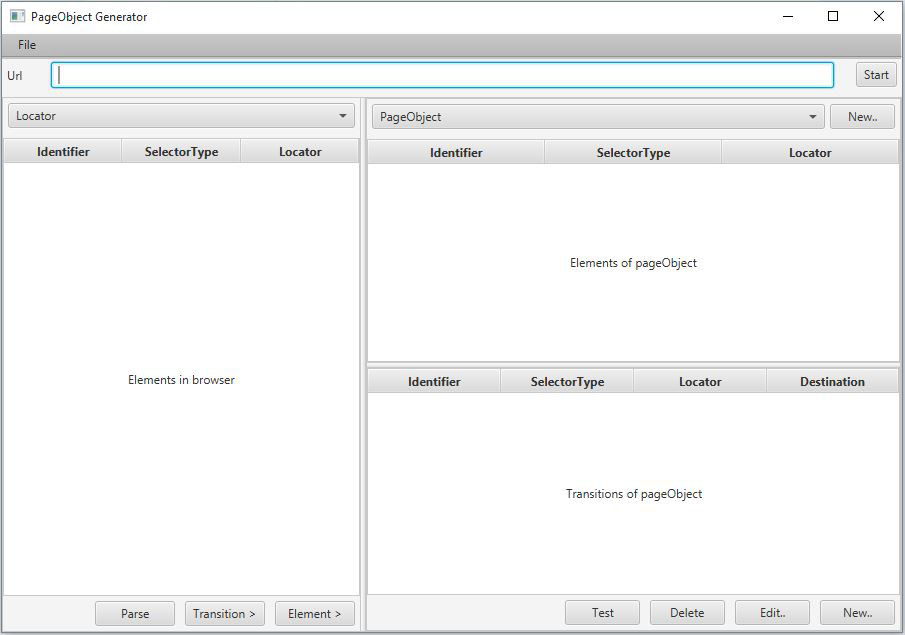
\includegraphics[scale=0.5]{img/poGeneratorMenu.JPG}\\
  \caption{SeleniPo - Page Object Generator - Menü}
  \label{fig:poGeneratorMenu}
\end{figure}

\subsection{Einordnung des Page Object Generator in den Gesamtkontext}
\label{sec:deploymentsicht}


Abbildung \ref{fig:deployment} zeigt die Einordnung des Page Object Generator in die Infrastruktur von it@M. Anhand dieser Abbildung soll gezeigt werden, in welchem Bezug sich der Generator zu einer zu testenden Webanwendung und dem späteren Testprojekt befindet.

\begin{figure}[htb]
  \centering  
  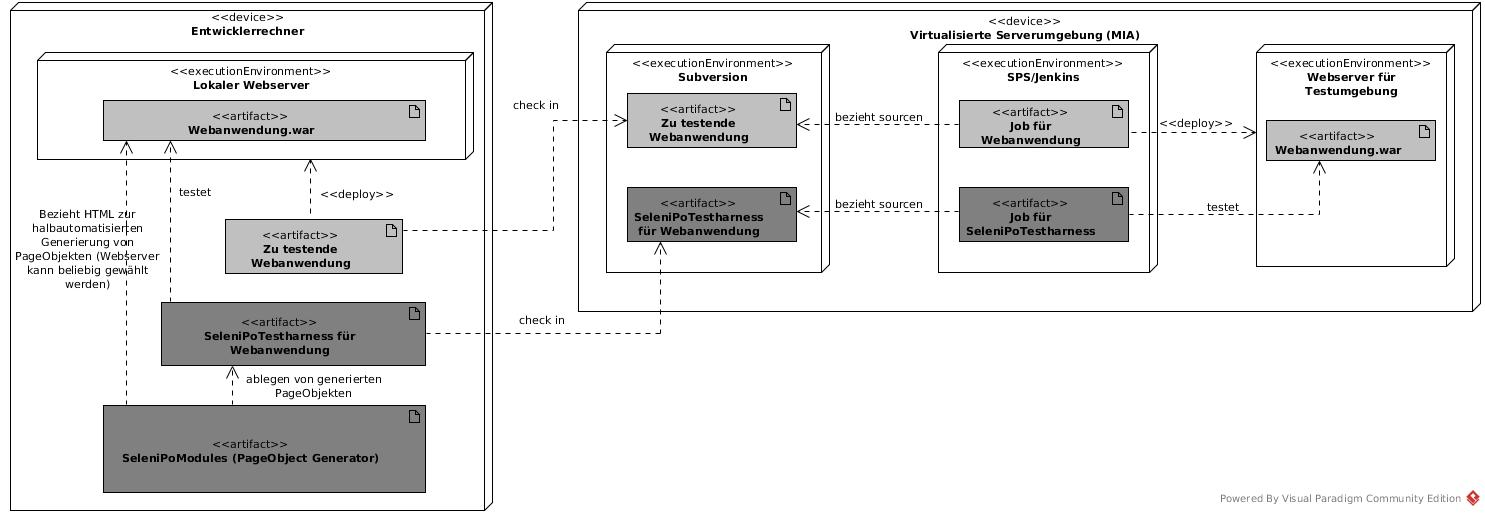
\includegraphics[scale=0.45]{img/Deployment.jpg}\\
  \caption{Einordnung des Page Object Generator in die Deploymentsicht}
  \label{fig:deployment}
\end{figure}

Zwei übergeordnete Teilbereiche werden unterschieden. Die virtualisierte Serverumgebung (MIA) und der lokale Rechner eines Entwicklers.\\
Auf der virtualisierten Serverumgebung werden die entwicklerübergreifenden Infrastrukturkomponenten, wie beispielsweise eine Versionsverwaltung, bereitgestellt. Unter dem Entwicklungsrechner ist der Arbeitsplatz eines einzelnen Projektteilnehmers zu verstehen.\\
Auf dem Entwicklungsrechner wird die zu testende Webanwendung entwickelt. Zu Testzwecken kann diese Anwendung, in ihrem aktuellen Entwicklungsstand, auf einem lokalen Webserver bereitgestellt werden.
Der lokale Rechner des Entwicklers ist darüber hinaus auch der Ort, an dem der Page Object Generator eingesetzt wird. Die vom Entwickler lokal bereitgestellte Webanwendung kann verwendet werden, um für die verschiedenen Seiten der zu testenden Anwendung Page Objects mit Hilfe des Generators zu erzeugen. Diese Page Objects werden in ein Test-Projekt abgelegt, in welchem später auch die Selenium-Testfälle entwickelt werden. In Abbildung \ref{fig:deployment} wird dieses Projekt als SeleniPoTestharness bezeichnet und kann vom Entwicklerteam entweder selbst erstellt oder als leeres Quickstart-Projekt vorgefertigt bezogen werden.\\ 
Mit Hilfe der Page Objects im Testharness können Testfälle entwickelt werden, die während der Erstellung auf dem lokalen Entwicklungsrechner, gegen die lokal bereitgestellte Webanwendung ausgeführt werden.\\
Über die virtualisierte Serverumgebung werden die lokal erstellten Ergebnisse zusammengeführt. 
Der Sourcecode der zu testende Webanwendung, sowie des SeleniPoTestharness, wird in einer Versionsverwaltung in der MIA abgelegt. Bei it@M kommt zu diesem Zweck \grq Subversion\grq\ zum Einsatz.\\
Über die Versionsverwaltung kann dann ein Integration Server bedient werden, der das Bauen, Bereitstellen und Testen der Webanwendung automatisiert. It@M verwendet hierfür den Continuous Integration Server \grq Jenkins\grq\ in Verbindung mit Maven und einem Artifactory.\\
Jenkins bezieht die jeweils aktuellen Sourcen für das Testprojekt und die Webanwendung aus der Versionsverwaltung. So kann regelmäßig eine aktuelle Version der Webanwendung gebaut und auf einem Testsystem in der virtuellen Serverumgebung bereitgestellt werden. Gegen dieses Testsystem können dann mit Hilfe des Jenkins-Servers die im Testharness entwickelten Selenium Testfälle zur Ausführung gebracht werden.



\subsection{Beispielhafter Ablauf bei der Benutzung des Page Object Generators}
\label{sec:moeglicher_ablauf_eines_standartanwendungsfall}

Abbildung \ref{fig:sequenz} zeigt auf hoher Abstraktionsebene einen Standardablauf bei der Benutzung des Page Object Generators.



\begin{figure}[htb]
  \centering  
  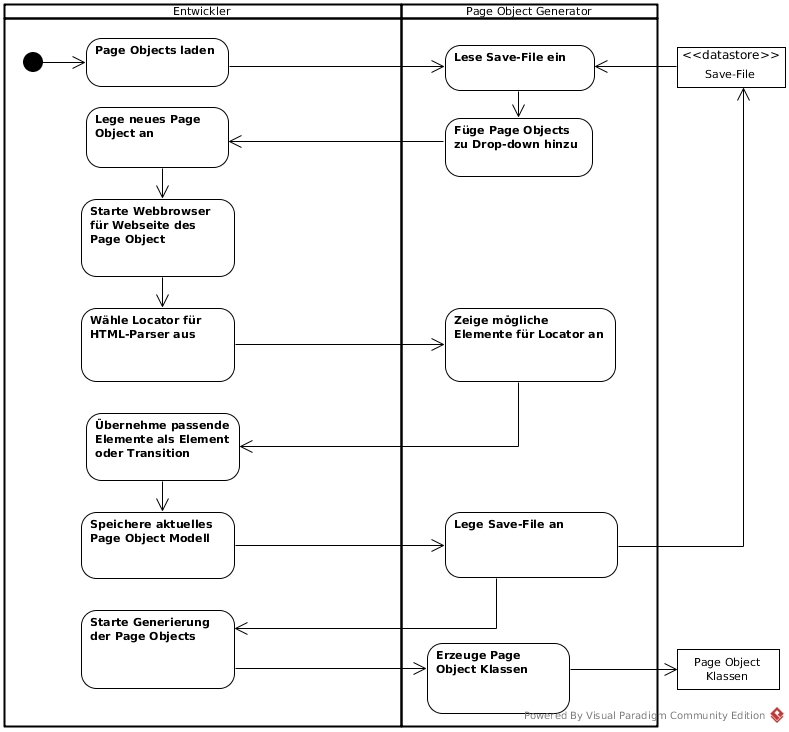
\includegraphics[scale=0.45]{img/Activitydiagram.jpg}\\
  \caption{Beispielhafter Ablauf bei der Benutzung des Page Object Generator}
  \label{fig:sequenz}
\end{figure}

Über das Menü (siehe Abbildung \ref{fig:poGeneratorMenu}) hat der Benutzer des Page Object Generators die Möglichkeit, einen bereits zuvor angelegten Zwischenstand des Page Object Modells aus einer Save-File zu laden. Die bereits angelegten Page Objects werden nach dem Laden im Dropdown-Menü im Bereich des Page Object Modells (siehe Abbildung \ref{fig:poGeneratorPo}) angezeigt. Der Benutzer hat nun die Möglichkeit, mit den bereits vorhandenen Page Objects weiterzuarbeiten oder ein neues Page Object anzulegen. Entscheidet er sich ein neues Page Object anzulegen, wird dies im Dropdown-Menü vorausgewählt angezeigt. Das Page Object kann nun manuell mit Elemente bzw. Transitionen befüllt werden.\\ Um das Page Object jedoch teilautomatisiert zu befüllen wird ein Webbrowser gestartet. Im Browser muss die Seite der Webanwendung aufgerufen werden, die dem aktuell ausgewählten Page Object entspricht. Mit dem Dropdown des HTML-Parser (siehe Abbildung \ref{fig:poGeneratorHtml}) wird die ausgewählte Webseite nach Elementen bzw. Transitionen durchsucht.
Passende Ergebnisse können dann in das ausgewählte Page Object übernommen und dort bei Bedarf noch einmal überarbeitet werden.
Der neu generierte Zwischenstand wird wiederum über das Menü gespeichert.\\
Um die Page Objects letztendlich als Code aus dem Modell zu erzeugen, kann über das Menü die Generierung gestartet werden. Bei richtiger Konfiguration des Page Object Generators muss dazu lediglich das Rootverzeichnis des entsprechenden Testprojektes als Zielort der Generierung gewählt werden.


\subsection{Anwendungsfälle des Page Object Generator}
\label{sec:page_object_generator_usecases}

Die konkreten Anwendungsfälle des Page Object Generators sind in Abbildung \ref{fig:use_case} dargestellt.

\begin{figure}[htb]
  \centering  
  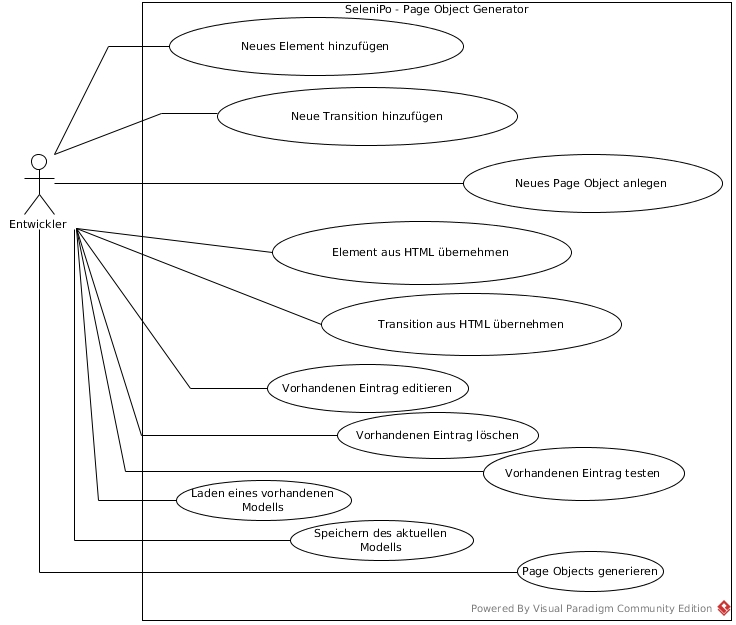
\includegraphics[scale=0.45]{img/Use-Cases.jpg}\\
  \caption{Anwendungsfälle des Page Object Generators}
  \label{fig:use_case}
\end{figure}

Eine detailierte Ausformulierung der Anwendungsfälle befindet sich im Anhang \ref{anhang:anwendungsfallbeschreibung}

\newpage

\subsection{Aufbau und technische Aspekte der Anwendung}
\label{sec:aufbau_des_systems}
In seiner internen Struktur ist der Page Object Generator in vier Module aufgeteilt, die unterschiedliche Aufgaben übernehmen. Diese Module sind auf Projektebene in einem übergeordneten Modul mit dem Namen \grq SeleniPoModules\grq\ zusammengefasst. Abbildung \ref{fig:component_diagramm} zeigt die verschiedenen Module und deren Abhängigkeiten zueinander.
Neben den Modulen des Page Object Generators zeigt Abbildung \ref{fig:component_diagramm} zusätzlich den SeleniPoTestharness, der dazu verwendet werden kann, die vom Page Object Generator erzeugten Klassen in einen ausführbaren Kontext zu stellen.\\
Im Folgenden wird auf die Aufgaben der einzelnen Module kurz näher eingegangen.

\begin{figure}[htb]
  \centering  
  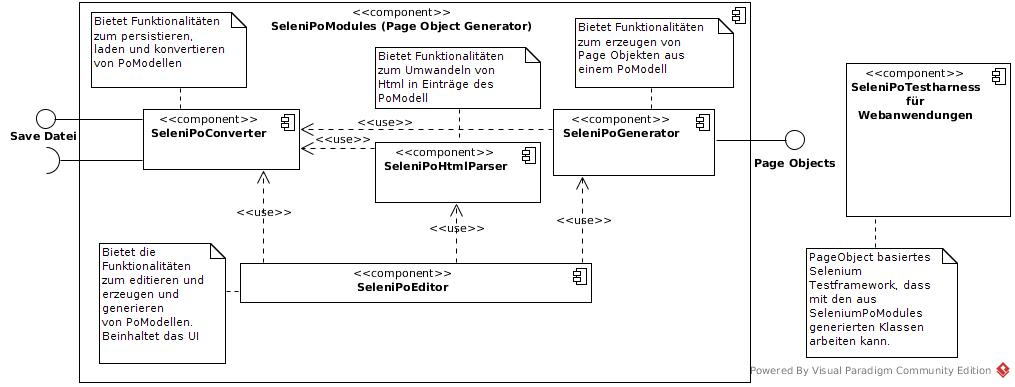
\includegraphics[scale=0.46]{img/ComponentDiagram.jpg}\\
  \caption{Module des Page Object Generators}
  \label{fig:component_diagramm}
\end{figure}

\subsubsection{SeleniPoEditor}
\label{sec:selenipoeditor}

Das zentrale Modul des Page Object Generators ist der SeleniPoEditor.
Ausgehend von diesem Modul werden die übrigen Module verwendet, um die in Kapitel \ref{sec:page_object_generator_usecases} vorgestellten Anwendungsfälle zu verwirklichen.
Das Modul SeleniPoEditor stellt dazu die grafische Benutzeroberfläche (GUI) der Anwendung bereit.
Als Technologie wird dazu JavaFX \cite{oracle_client_2015} verwendet, das mit der Java Version 8 Einzug in den Oracle JDK gefunden hat. \\
Um eine hohe Wartbarkeit dieser Komponente zu gewährleisten, wurde die GUI nach dem Model-View-Controller Prinzip verwirklicht.
Das Modell besteht aus einem anwendungsspezifischem Java Objekt, welches eine Liste von Page Objekten mit deren zugehörigen Attributen darstellt.
Für die View wird die XML-basierte Sprache FXML verwendet, um losgelöst von der Applikationslogik die Struktur der Benutzeroberfläche zu beschreiben.
Der Controller besteht aus Java Klassen, mit deren Hilfe das Verhalten der GUI bei Benutzerinteraktion beschrieben wird.
Komplexere Logik, wie beispielsweise das Generieren der fertigen Page Object Klassen wird mittels Services durch die übrigen Modulen bereitgestellt.\\
Das Verhalten der GUI wird über einen Zustandsautomaten gesteuert.
Interaktionen mit der Oberfläche beeinflussen den Zustand, in dem sich die Anwendung befindet. Je nach Zustand variieren die Aktionen, die von den verschiedenen Buttons der Anwendung ausgelöst werden.
Mit Hilfe dieses Vorgehens kann beispielsweise beim Editieren nach der Auswahl eines Elements, ein anderer Dialog angezeigt werden, als nach der Auswahl einer Transition.
Die verschiedenen Zustände der GUI, sowie die Events, die in diesen Zuständen verarbeitet werden, sind im Anhang \ref{sec:zustände_des_page_object_generator} über einen erweiterten endlichen Automaten dargestellt.

\subsubsection{SeleniPoConverter}
\label{sec:selenipoconverter}
Das Modul SeleniPoConverter dient der Verwaltung des internen Modells des Page Object Generators. In dieser Komponente wird einerseits das Modell der Anwendung definiert, andererseits werden Services für andere Module bereitgestellt, um mit diesem Modell zu arbeiten.
Abbildung \ref{fig:simple_model} zeigt die Interface-Stuktur, welche das Modell abbildet.

\begin{figure}[htb]
  \centering  
  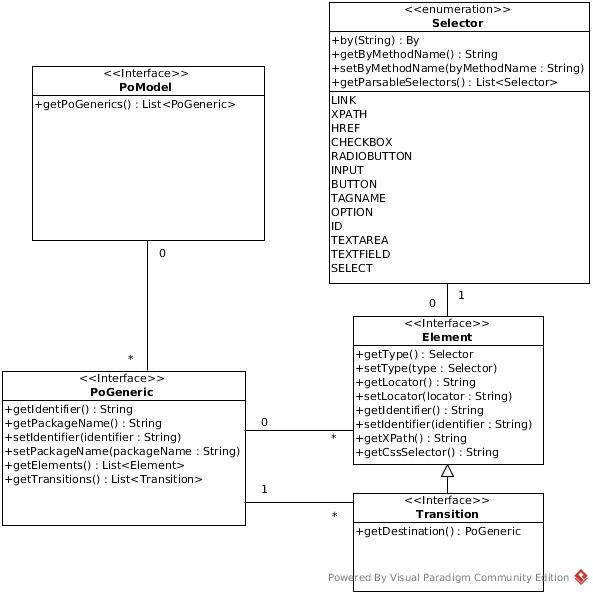
\includegraphics[scale=0.46]{img/SimpleModel.jpg}\\
  \caption{Vereinfachte Struktur des internen Modells des Page Object Generators}
  \label{fig:simple_model}
\end{figure}

Kern des Modells ist das Interface PoModel, welches eine Liste von PoGenerics beinhaltet. Ein PoGeneric repräsentiert die Informationen, die benötigt werden, um eine einzelne Page Object Klasse zu erzeugen. Dementsprechend vereint dieses Interface eine Menge an Elementen und Transitionen.
Ein Element steht dabei für eine beliebige Komponente einer Webseite, wie beispielsweise ein Eingabefeld.
Transitionen sind von Elementen abgeleitet. Es handelt sich also um eine speziellere Form von Elementen. Mit Hilfe von Transitionen ist es möglich, auch die dynamische Komponente einer Webseite in Form von Seitenübergängen abzubilden. Als Transition werden all die Komponenten einer Webseite bezeichnet, die einen Übergang auf ein neues Page Object auslösen. Im Gegensatz zu Elementen bieten Transitionen daher noch ein Page Object Ziel mit an. Über die Methode \grq getDestination()\grq\ kann dieses Page Object Ziel erfragt wrerden\\
Sowohl Elemente als auch Transitionen werden über eine Selektor-Enumeration genauer definiert.
Der Selektor gibt für ein Element im Modell an, welche Suchstrategie beim Auflösen des Lokators gegen die Webseite verwendet werden soll.
Die verfügbaren Strategien werden durch die verschiedenen Aufzählungstypen der Enumeration festgelegt.\\
Die Kerninformation zum Adressieren eines Elements auf der Webseite bildet der Lokator. Vom Generator wird diese Variable mit einem Wert befüllt, der charakteristisch für das zu adressierende Element ist. Je nach Element handelt es sich hierbei oft um ein HTML-Attribut, wie beispielsweise id- oder value-Attribute des entsprechenden HTML-Tags.\\
In Verbindung mit dem ausgewählten Selektor kann über die Klasse ByFactory aus dem Lokator ein repräsentativer XPath-Ausdruck bzw. CSS-Selektor für das Element erzeugt werden. Im Kapitel \ref{sec:selenipotestharness} wird darauf näher eingegangen.\\
Abbildung \ref{fig:simple_model} zeigt lediglich die Interface-Struktur des zugrunde liegenden Modells. Der Page Object Generator kennt zwei konkrete Implementierungen. Das vollständige Modell ist in Anhang \ref{anhang:vollständiges_technisches_modell} abgebildet.\\
Zwei verschiedene Implementierungen sind notwendig, da JavaFX und XStream \cite{joe_walnes_xstream_2015}, welches für die Persistierung in XML verwendet wird, unterschiedliche Anforderungen an das Modell stellen. JavaFX benötigt spezielle Datentypen. Anstelle einer gewöhnlichen List wird beispielsweise eine ObservableList verwendet, um die View der GUI automatisch mit dem Modell synchron zu halten. Diese Datentypen können von XStream aufgrund eines fehlenden argumentlosen Konstruktors jedoch nicht mehr deserialisiert werden.
Dementsprechend werden vom Converter eine Reihe von Services bereitgestellt, die das Wandeln des Modells in zwei Implementierungen ermöglicht. Eine Implementierung kann verwendet werden, um das Modell zu persistieren und wieder zu deserialisieren. Die Zweite Implementierung wird verwendet um im Umfeld von JavaFX zu arbeiten.\\
Abbildung \ref{fig:converter_service} zeigt alle vom Converter bereitgestellten Services. 

\begin{figure}[htb]
  \centering  
  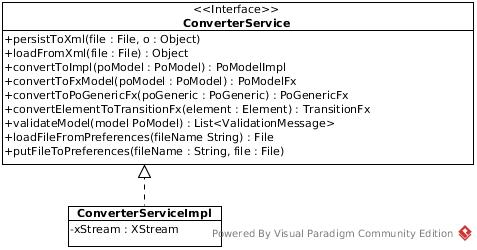
\includegraphics[scale=0.5]{img/ConverterService.jpg}\\
  \caption{Services, die von SeleniPoConverter bereitgestellt werden}
  \label{fig:converter_service}
\end{figure}

Neben den Services zum Wandeln des Modells wird in diesem Modul auch die Funktionalität zum Speichern und Laden, sowie zur fachlichen Validierung bereitgestellt.
Zusätzlich wird die Möglichkeit geboten, benutzerspezifische Informationen, wie beispielsweise der Pfad zur zuletzt verwendeten Save-File, in den Properties des Anwenders abzulegen.


\subsubsection{SeleniPoHtmlParser}
\label{sec:selenipohtmlparser}

Das SeleniPoHtmlParser Modul beinhaltet die Funktionalität zum teilautomatisierten befüllen der Page Objects mit Elementen bzw. Transitionen.
Das Modul stellt dazu eine Methode bereit, die es ermöglicht HTML-Quelltext anhand von einem übergebenen Selektor auszuwerten.
Abbildung \ref{fig:html_service} zeigt das Klassendiagramm für diesen Service.

\begin{figure}[htb]
  \centering  
  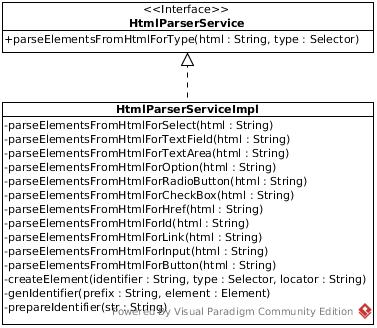
\includegraphics[scale=0.5]{img/HtmlParserService.jpg}\\
  \caption{Services, die von SeleniPoHtmlParser bereitgestellt werden}
  \label{fig:html_service}
\end{figure}

Der benötigte HTML-Quelltext wird direkt aus einem Webbrowser bezogen, der über die Benutzeroberfläche der Anwendung gestartet werden kann.
Das Parsing des Quelltextes übernimmt die freie Bibliothek jsoup \cite{hedley_jsoup_2015}.
Für jeden in der Selektor-Enumeration (siehe Kapitel \ref{sec:selenipoconverter}) definierten Aufzählungstypen wurde dazu eine eigene Strategie implementiert. 
Die für die jeweiligen Selektoren implementierte Filterstrategie orientiert sich an der Strategie, die später in den Testfällen verwendet wird, um die Elemente auf der Webseite zu adressieren.\\
Listing \ref{lst:parserLINK} zeigt beispielhaft die Implementierung für den Aufzählungstypen LINK, der Links auswählt, welche eines der HTML-Attribute id, text oder title besitzen:
\begin{lstlisting}[caption={Parser für den Aufzählungstypen LINK},label={lst:parserLINK}]
 	/**
	 * Sucht nach Links fuer die vorhanden ist: id or text or title
	 *
	 * @param html Quelltext der zu untersuchenden Seite
	 * @return PoGeneric - neues Page Object mit den gefundenen Elementen
	 */
	private PoGeneric parseElementsFromHtmlForLink(String html) {
		final String PREFIX = "a";
		PoGeneric poGeneric = new PoGenericImpl();
		Document doc = Jsoup.parse(html);
		Elements elements = doc.select("a");
		for (Element element : elements) {
			if (element.hasAttr("id")) {
				de.muenchen.selenipo.Element createdElement = createElement(
						genIdentefier(PREFIX, element), Selector.LINK,
						element.attr("id"));
				poGeneric.getElements().add(createdElement);
			}
			else if (element.hasText()) {
				de.muenchen.selenipo.Element createdElement = createElement(
						genIdentefier(PREFIX, element), Selector.LINK,
						element.text());
				poGeneric.getElements().add(createdElement);
			}
			else if (element.hasAttr("title")) {
				de.muenchen.selenipo.Element createdElement = createElement(
						genIdentefier(PREFIX, element), Selector.LINK,
						element.attr("title"));
				poGeneric.getElements().add(createdElement);
			}
		}
		return poGeneric;
	}
  }
  
\end{lstlisting} 

Dieses Vorgehen hat den Nachteil, dass die Möglichkeit besteht, Elemente zu verwerfen, die vom Benutzer für den ausgewählten Filter zwar erwartet werden, den implementierten Filterkriterien jedoch nicht entsprechen.
Im Beispiel aus Listing \ref{lst:parserLINK} wären das alle Links, für die weder das Attribut id, text oder title gesetzt ist.\\
Durch dieses Vorgehen ist allerdings sichergestellt, dass für einen untersuchten Selektor nur Elemente zur Auswahl gestellt werden, die in den späteren Testfällen auch aufgelöst werden können. So wird verhindert, dass über die Page Objects Elemente bereitgestellt werden, die später in den Testfällen zu Fehlern führen.\\
Die Palette der vorgefertigten Filter deckt einen großen Teil der in HTML vorhandenen Elemente bereits ab. Sollte es dennoch vorkommen, dass Elemente über die existierenden Selektoren nicht erreicht werden, besteht die Möglichkeit mit Hilfe des Selektors XPATH, Elemente über einen eigenen XPath-Ausdruck anzusprechen.



\subsubsection{SeleniPoGenerator}
\label{sec:selenipogenerator}
Das Modul SeleniPoGenerator ermöglicht es, aus einem Modell des SeleniPoConverters, Page Object Klassen zu generieren.
Abbildung \ref{fig:generator_service} zeigt die Services, die von diesem Modul angeboten werden.

\begin{figure}[htb]
  \centering  
  \includegraphics[scale=0.5]{img/SelenipoGenerator.jpg}\\
  \caption{Services die von SeleniPoHtmlParser bereitgestellt werden}
  \label{fig:generator_service}
\end{figure}

Für die Generierung des Codes aus dem Modell der Anwendung wird die Template-Engine Velocity \cite{apache_software_foundation_apache_2015} verwendet.
Mit Hilfe von Velocity kann ein beliebiges Modell der Anwendung über vordefinierte Templates in die gewünschten Page Object Klassen gewandelt werden.
Diese Templates können vom Benutzer des Page Object Generators beliebig editiert werden. So ist es möglich, die im Modell der Anwendung hinterlegten Informationen in jede, vom Anwender gewünschte Form aufzubereiten. Anhang \ref{anhang:beispiel_velocity_template} zeigt als Beispiel den Templatevorschlag, der im Rahmen dieser Arbeit im Page Object Generator verwendet wird.\\
Für jedes Page Object im Modell werden jeweils zwei Klassen erzeugt. Eine Klasse, welche die gesamte generierte Logik enthält, sowie eine weitere Klasse, welche abgesehen von einem Konstruktor leer ist und von dieser Klasse ableitet. 
Die komplexe Klasse wird im folgenden als \grq PageObject\_Generated\grq\ bezeichnet. Das zugehörige Template befindet sich in Listing \ref{lst:template_pogenerated}. Die
bis auf den Konstruktor leere Klasse wird im folgenden als \grq PageObject\_Dynamisch\grq\ bezeichnet und ist im Template, in Listing \ref{lst:template_poeditable} dargestellt.\\
Abbildung \ref{fig:postruktur} zeigt die Abhängigkeit zwischen den beiden zu generierenden Klassen.

\begin{figure}[htb]
  \centering  
  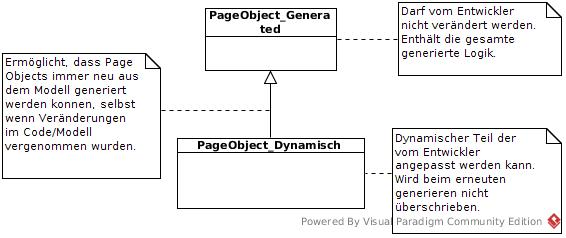
\includegraphics[scale=0.6]{img/postruktur.jpg}\\
  \caption{Abhängigkeit zwischen dem generierten und dem dynamischen Teil eines Page Objects}
  \label{fig:postruktur}
\end{figure}
 
Mit Hilfe der Aufteilung eines Page Objects in zwei Klassen soll verhindert werden, dass bei mehrmaligem Generieren des gleichen Page Objects Änderungen, die vom Testentwickler im Code vorgenommen wurden, überschrieben werden. Als Konvention gilt daher, dass Änderungen durch den Entwickler nur im PageObject\_Dynamisch vorgenommen werden dürfen. Der generierte Teil des Page Objects darf vom Entwickler nicht verändert werden.
Bei einem erneuten generieren der Page Objects werden lediglich die PageObject\_Generated überschrieben, der dynamische Teil bleibt unangetastet.
Dadurch ist sichergestellt, dass Änderungen, die im dynamischen Teil geschehen nicht überschrieben werden, jedoch Anpassungen die über den Page Object Generator vorgenommen wurden, Einzug in den generierten Teil finden können.
Page Objects können so über die gesamte Projektlaufzeit iterativ im Page Object Generator aufgebaut werden und müssen nicht bereits zu Beginn im finalen Zustand modelliert werden.\\
Der Ort an dem die fertigen Page Objects abgelegt werden, ist über eine Konfigurationsdatei und eine Variable in den Page Objects einstellbar. 
Abbildung \ref{fig:packagepath} stellt grafisch dar, wie die endgültige Paket-Struktur eines Page Objects gebildet wird.
\begin{figure}[htb]
  \centering  
  \includegraphics[scale=0.8]{img/packagePath.png}\\
  \caption{Erzeugen der Paket-Struktur eines Page Object}
  \label{fig:packagepath}
\end{figure}
In der Grundkonfiguration wird der generierte Teil eines Page Objects unterhalb des Ordners \grq src.main.generated\grq\ abgelegt. Der dynamische Teil befindet unterhalb von \grq src.main.java\grq.
Diese Strukturierung bildet die getroffene Konvention ab, dass bei Verwendung der Page Objects der dynamische teil als Instanz in den Testfällen verwendet wird, der generierte Teil aber nicht editiert werden darf.
Ausgehend von diesen Verzeichnissen ist es über die Konfiguration möglich, den Pfad weiter zu verfeinern. So kann konfiguriert werden, dass der generierte Teil eines Page Objects immer im Paket \grq de.muenchen.selenipo.po\grq\ abgelegt wird, der dynamische im Paket \grq de.muenchen.selenipo.po\grq.\\
Während der Erstellung im Page Object Generator kann auf Ebene der Page Objects eine weitere Verfeinerung der Struktur vorgenommen werden. Ausgehend von den global konfigurierten Ziel-Paketen ist es so möglich, jedes Page Object in ein beliebiges Paket abzulegen.
Bei richtiger Konfiguration kann dann für die Generierung der Klassen, einfach das Rootverzeichnis des Testprojektes ausgewählt werden.

\subsubsection{SeleniPoTestharness}
\label{sec:selenipotestharness}

Im Rahmen dieser Arbeit wurde auch ein Testprojekt entwickelt, welches mit den Page Objects, die über den Page Object Generator erzeugt wurden, arbeiten kann.
Das Testprojekt wird im folgenden als Testharness bezeichnet.\\
Damit Testharness und Page Object Generator zusammenarbeiten können, muss die Struktur der Templates des Generators mit der Struktur des Testharness zusammenpassen.
Die Struktur der Templates kann vom Benutzer des Page Object Generators jederzeit angepasst werden. Prinzipiell kann dadurch jede Struktur eines Testharness unterstützt werden.\\
Um mit den Templates, die im Rahmen dieser Arbeit entwickelt wurden, zusammenzuarbeiten, muss der Testharness allerdings einige Anforderungen erfüllen.
Abbildung \ref{fig:strukturTestharness} zeigt die Page Object Struktur, die sowohl in den Templates als auch im Testharness verwendet wird.\\
\begin{figure}[htb]
  \centering  
  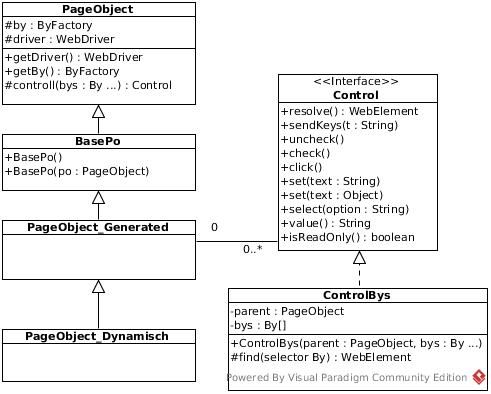
\includegraphics[scale=0.49]{img/strukturTestharness.jpg}\\
  \caption{Page Object Struktur des Testharness}
  \label{fig:strukturTestharness}
\end{figure}

Die Wurzel der Vererbungshierarchie eines Page Objects im Testharness bildet die Klasse PageObject. Die Klasse PageObject beinhaltet den Selenium WebDriver. Neben dem WebDriver enthält die Klasse PageObject noch eine zusätzliche Kernkomponente, die Klasse ByFactory. Diese Klasse zählt nicht zum Standard bei der Verwendung des Page Object Pattern sondern ist spezifisch für die in dieser Arbeit verwirklichte Implementierung eines Testharness.
Die Helferklasse ByFactory ermöglicht es in einfacher Art, komplexe \grq org.openqa.selenium.By\grq -Ausdrücke zu erzeugen. Die erzeugten Ausdrücke werden verwendet, um über den WebDriver Elemente auf der Webseite zu lokalisieren. Als Übergabe erhält die Factory dazu einen einfachen Lokator-String, der beispielsweise dem value- oder id-Attribut des gesuchten HTML-Tags entspricht. Die Klasse ByFactory ist mit dem Page Object Generator abgestimmt. Für jeden Selektor des Generators gibt es eine entsprechende Factory-Methode. Die vom Generator erzeugten Lokatoren sind so gewählt, dass sie von der ByFactory interpretiert werden können. Damit ist sichergestellt, dass ein vom Generator erzeugter Lokator von der entsprechenden Factory-Methode aufgelöst werden kann.\\
Die Verwendung der Factory-Klasse bringt den Vorteil, dass komplexe XPath Ausdrücke einfach erzeugt sowie gekapselt und lesbar in den Page Objects abgelegt werden können. 
Das Modell des Generators bietet auch die Möglichkeit die bereits aufgelösten Ausdrücke, ohne die zusätzliche Verwendung der ByFactory, zu erhalten.
Mit den Methoden  \grq Element.getXPath()\grq\ bzw.  \grq Element.getCssSelector()\grq\ können je nach verwendetem Selektor, der XPath bzw. der CssSelector als String erfragt werden. \\
Die Klasse BasePo ist das nächste Kind in der Vererbungshierarchie. Als einzige Klasse bietet BasePo einen parameterlosen Konstruktor und bildet somit, bei der Verwendung der Page Objekts, den Einstiegspunkt in einen Testfall. Bei der konstruktorlosen Initialisierung des BasePo wird ein neuer WebDriver erzeugt, der auf einer über die Konfiguration hinterlegbaren Adresse startet.
Alle weiteren Page Objects erhalten bei der Instanziierung als Übergabe ein bereits vorhandenes Page Object, aus dem der WebDriver übernommen werden kann.
Damit kann der Zustand des WebDrivers innerhalb eines Testfalls von Page Object zu Page Object übergeben werden.\\
Ausgehend von der Klasse BasePo erben die vom Page Object Generator erzeugten Klassen, PageObject\_Generated und PageObject\_Dynamisch (siehe Kapitel \ref{sec:selenipogenerator}).
Die verschiedenen Elemente der Webseite werden im Page Object als Implementierung des Interfaces Control angeboten.
Die Klasse ControlBys implementiert dieses Interface und kapselt ein Selenium WebElement. Als Referenz gegen die Webseite wird bei der Instanziierung ein By-Ausdruck übergeben, der mittels ByFactory erzeugt werden kann.
Für die Interaktion mit dem referenzierten Element bietet die Klasse eine Vielzahl von Methoden an. Eine davon ist die Methode \grq Control.resolve()\grq, welche das gekapselte WebElement zurückliefert.\\
Die Kapselung eines WebElements in die Klasse ControlBys hat den Vorteil, dass WebElemente in einem PageObject als globale Variablen geführt werden können.
Die Klasse ControlBys verhindert, dass ein WebElement sofort bei der Instanziierung eines PageObject gegen die geladene Webseite im Webdriver aufgelöst wird. Erst beim Aufruf einer Methode wird der übergebene By-Ausdruck verwendet, um das eigentliche WebElement über die WebDriver-Methode \grq findElement()\grq\ zu erhalten.
So wird verhindert, dass ein Page Object bereits bei der Instanziierung versucht, Elemente auf der Webseite abzufragen, die möglicherweise noch gar nicht geladen sind oder erst durch vorangegangene Interaktion erreichbar gemacht werden müssen.\\ Zum einfachen Erzeugen von Controls bietet die Klasse PageObject die statische Methode \grq control(bys : By ...)\grq\ an, die auch in den Templates verwendet wird.


\section{Praxistest}
Um im Praxisbetrieb erste Erfahrungen mit dem Page Object Generator zu sammeln, wurde eine frühe Version des Generators dazu verwendet, Page Objects für ein bereits etabliertes Projekt mit geringer Testabdeckung zu erzeugen.\\
Für das System zur Verwaltung von Schulversäumnissen in Schulen der Stadt München sollten Systemtests mit Hilfe des Selenium WebDrivers erstellt werden. Mit Hilfe des Page Object Generators wurden die benötigten Page Objects erzeugt. Der Fokus im ersten Praxistest wurde darauf gelegt, Erfahrungen zu sammeln, wie intuitiv die Bedienung des Page Object Generators für neue Anwender nach einer kurzen Einweisung ist. Die Erkenntnisse, die dabei gesammelt wurden, lieferten ma\ss gebliche Hinweise, die vor allem zu großen Verbesserungen im Bereich der Benutzerfreundlichkeit führten.\\
Wichtige Bereiche der Anwendung sind aufgrund des Feedbacks nun über Tastatureingaben zu steuern und nicht mehr nur exklusiv über die in der GUI angebotenen Interaktionskomponenten.\\
Darüber hinaus hat sich gezeigt, dass in der Regel eine Vielzahl von Elementen und Transitionen für ein Page Object auf einmal übernommen werden können und nicht, wie zuvor angenommen, immer nur einzelne Einträge. Die Übernahme von Elementen und Transitionen ist daher nicht mehr nur auf einzelne Ergebnisse des Parsers beschränkt. Per Mehrfachauswahl können nun auch eine Vielzahl von Treffern in einem Schritt übernommen werden.\\
Die Anwendung in der Praxis hat auch gezeigt, dass das Laden, Speichern und Generieren von Page Objects Aktionen sind, die häufiger ausgeführt werden, als zu Beginn erwartet.
Aufgrund dieser Erkenntnis wurde die Anwendung dahingehend verbessert, dass sie sich den letzten, vom Benutzer für die jeweilige Aktion ausgewählten Pfad, merkt. Lange Navigationswege bei der Auswahl der Zielordner können so vermieden werden.\\
Die genannten Veränderungen sind nur einige von einer Vielzahl von Verbesserungen, die durch den ersten Praxistest des Page Object Generators vorgenommen werden konnten.\\
Mit der überarbeiteten Version wurde ein zweiter Praxistest durchgeführt. In diesem Testbetrieb sollten für die Anwendung zum Erstellen der Jahresstatistiken der Kindertagesstätten der Stadt München Page Objects erzeugt werden.
Die Verbesserungen aus dem ersten Praxistest wurden gut angenommen. Die Bereiche die bei der Bedienung zuvor noch Probleme verursachten, zeigten nun intuitive Bedienbarkeit.
Der zweite Praxistest zeigte vor allem Bereiche im Page Object Generator auf, die im Hinblick auf eine höhere Flexibilität verbessert werden könnten.\\
Für die Generierung der eindeutigen Namen von Elementen und Transitionen werden in einem fest vorgegebenem Algorithmus die HTML-Attribute des jeweiligen HTML-Tags ausgewertet. Das gewählte Vorgehen liefert nicht immer sinnvolle Namen. In ungünstigen Konstellationen kann es vorkommen, dass der gleiche Wert mehrmals erzeugt wird, was zu unnötigem Mehraufwand bei der Überarbeitung der Namen führt.\\
Darüber hinaus hat sich gezeigt, dass die Aufteilung der Page Objects in einen generierten und einen dynamischen Teil, wie in Kapitel \ref{sec:selenipogenerator} beschrieben, nicht von allen Testanwendern intuitiv angenommen wird.
Auch wenn diese Aufteilung als sinnvoll erachtet wird, bietet es sich an dem Benutzer die Entscheidungsfreiheit zu überlassen, die Generierung des dynamischen Teils zu verhindern.\\
Auch bei der Erzeugung der Paket-Struktur, wie in Abbildung \ref{fig:packagepath} gezeigt, wurde eine zu eingeschränkte Konfigurierbarkeit bemängelt.
Sowohl für den dynamischen als auch für den generierten Teil eines Page Objects wird die selbe Variable zum Erzeugen des Pfades unterhalb von \grq src.main.java\grq\ bzw. \grq src.main.generated\grq\ verwendet. Ein Ablegen des dynamischen und des generierten Teil eines Page Objects in gänzlich verschiedenen Paketen ist damit nicht möglich.\\
Abgesehen von den Verbesserungsvorschlägen des ersten und zweiten Praxistests wurde der Page Object Generator in beiden Prüfungen von den Anwendern durchwegs als positiv bewertet. Die Generierung der Page Objects wurde als Arbeitserleichterung empfunden, welche eine Zeitersparnis im Vergleich zum manuellen Erzeugen mit sich bringt. Die Zeitdifferenz zum manuellen Erstellen der Page Objects, wurde in den Praxistests allerdings nicht wissenschaftlich gemessen und überprüft.





%Verzeichnis aller Bilder
\newpage
\listoffigures
\listoftables

%Literaturverzeichnis
\newpage
\bibliographystyle{alphadin}
\bibliography{Literatur}

\end{document}
